%%%%%%%%%%%%%%%%%%%%%%%%%%%%%%%%%%%%%%%%%%%%%%%%%%%%%%%%%%%%%%%%%%%%%%%%%%%%%%%%%%%%%%%%%%%%%%%%%%%%%%%%%%%%%%%%%%%%
%
% Masterarbeit im Fachbereich 1
% Systems Engineering - HTW Berlin
% 
% Thema:
% Lorem Ipsum
%
% \newcommand{\draftdate}{140910}
% \newcommand{\rev}{108}
% %
\newcommand{\thesisopening}{05. Januar 2015}
\newcommand{\thesisclosing}{16. März 2015}
\newcommand{\thesisrelease}{16. März 2015}
%%%%%%%%%%%%%%%%%%%%%%%%%%%%%%%%%%%%%%%%%%%%%%%%%%%%%%%%%%%%%%%%%%%%%%%%%%%%%%%%%%%%%%%%%%%%%%%%%%%%%%%%%%%%%%%%%%%%
%%%
%%
%





%%%%%%%%%%%%%%%%%%%%%%%%%%%%%%%%%%%%%%%%%%%%%%%%%%%%%%%%%%%%%%%%%%%%%%%%%%%%%%%%%%%%%%%%%%%%%%%%%%%%%%%%%%%%%%%%%%%%
%%%%%%%%%%%%%%%%%%%%%%%%%%%%%%%% D O K U M E N T K O N F I G U R A T I O N E N %%%%%%%%%%%%%%%%%%%%%%%%%%%%%%%%%%%%%
%%%%%%%%%%%%%%%%%%%%%%%%%%%%%%%%%%%%%%%%%%%%%%%%%%%%%%%%%%%%%%%%%%%%%%%%%%%%%%%%%%%%%%%%%%%%%%%%%%%%%%%%%%%%%%%%%%%%
%
%%
%%% 
% Dokumentformatierung
\documentclass
[a4paper,german,
12pt												% ersatzweise 12pt, wenn mehr Seiten entstehen sollen
]
{scrreprt}
%%%
%
%%%%%%%%%%%%%%%%%%%%%%%%%%%%%%%%%%%%%% P A C K A G E S %%%%%%%%%%%%%%%%%%%%%%%%%%%%%%%%%%%%%%%%%
%
%%% Textformatierung %%%
%

\usepackage[onehalfspacing]{setspace}				% Zeilenabstand bestimmen
\usepackage[table]{xcolor}							% farbiger Text
\usepackage{colortbl}								% Tabellen mit Hintergrundfarben versehen
\usepackage{lettrine}								% Kapitelbeginn mit großem Buchstaben
\usepackage{fancybox}								% Schattierungen und Rahmen für Grafiken
\usepackage{wrapfig}								% Paket zur Positionierung von Grafiken
\usepackage{capt-of}								% Untertitel von Abbildungen, Tabellen usw. in Gleitumgebung
\usepackage[ngerman]{babel,translator}				% Silbentrennung nach der neuen deutschen Rechtschreibung, z.B.: Sys-tem
\usepackage{paralist}								% Kompakte Aufzaehlungen erstellen
\usepackage[bottom]{footmisc}							% Fussnoten am Seitenende
\usepackage{fancyhdr}								% Kopf- und Fußzeilenformatierung
\usepackage{pdfpages}								% für die Einbindung kompletter pdf-*Seiten*
\usepackage{eso-pic}								% Wasserzeichen z.B. "`ENTWURF"' auf .pdf erzeugen
\usepackage[hyphens]{url}							% für \url{http://www}, Option hyp erlaubt auch Umbruch nach "-"
\usepackage[numbers,square]{natbib}					% Für \setlength{\bibsep}{3mm}; square macht eckige Klammern
\usepackage{bibgerm}								% Styles für Literaturverzeichnisse
\usepackage{titlesec, blindtext, color}				% Styles für Kapitelüberschriften
\usepackage[printonlyused,withpage]{acronym}		% Abkürzungsverzeichnis
%
\usepackage{tabularx}
\usepackage[utf8]{inputenc}							% Zeichensatz, ermöglicht die direkte Eingabe von Umlauten im Editor
\usepackage[T1]{fontenc}							% Optimiert Umlautverwendung
\usepackage{lmodern}								% Schriften aufgrund von 'fontenc' glätten
\usepackage{graphicx}								% Einbindung von Grafiken (pdf, png, jpg)
\usepackage{float}									% bietet Option [H] für bombenfestes Verankern
\usepackage{enumerate}								% verbessert Aufzählungen
\usepackage{expdlist}								% erweiterter Funktionssatz für description
\usepackage{chngcntr}								% Konfiguration des Fußnotenzählers ermöglichen
\usepackage{array}									% für Tabellen: bindet tabular-Umgebung ein
\usepackage{parskip}								% zw. Absätzen: eine knappe Leerzeile statt hängender Einzüge
\usepackage[right]{eurosym}							% Eurosymbol
\usepackage{makeidx}								% Package zur Indexerstellung
\usepackage{multicol}								% zur Indexerstellung in zwei Spalten
\usepackage{multirow}								% Verbinden von Zellen in Tabellen
\usepackage{booktabs}								% Tabellenlayout anpassen
\usepackage{longtable}								% Tabellen über mehrere Seiten strecken
\usepackage{chngcntr}								% Nummeriegung der Abbildungen beeinflussen (z.B. nach Kapitel/fortlaufend)
\usepackage[outercaption]{sidecap}					% Bildunterschriften rechts neben der Abbildung positionieren
\usepackage[bf]{caption}							% Kuerzel und Nummerierung von Bildunterschriften "`fett"' schreiben
\usepackage{amssymb}								% Erweiterte Symboldarstellung
\usepackage{times}
\usepackage{listings}
%%
% Packagehinweise
% Folgende Packete müssen zusätzlich von MiKTeX bereitgestellt werden:
% setspace, xcolor, colortbl, lettrine, fancybox, wrapfig, capt-of, translator, paralist, expdlist, footmisc, fancyhdr, pdfpages, eso-pic, url,
% natbib, bibgerm, titlesec, blindtext, acronym, suffix, xstring, glossaries, etoolbox, textcase, xfor, datatool-base, substr, fp, supertabular,
% mptopdf
%%
%%%%%%%%%% NEW FOR TESTING %%%%%%%%%%
%
%%


%%LISTINGS SETTINGS
\definecolor{mygreen}{rgb}{0,0.6,0}
\definecolor{mygray}{rgb}{0.5,0.5,0.5}
\definecolor{mymauve}{rgb}{0.58,0,0.82}


\lstset{ %
  backgroundcolor=\color{white},   % choose the background color; you must add \usepackage{color} or \usepackage{xcolor}
  basicstyle=\footnotesize,        % the size of the fonts that are used for the code
  breakatwhitespace=false,         % sets if automatic breaks should only happen at whitespace
  breaklines=true,                 % sets automatic line breaking
  captionpos=b,                    % sets the caption-position to bottom
  commentstyle=\color{mygreen},    % comment style
  deletekeywords={...},            % if you want to delete keywords from the given language
  escapeinside={\%*}{*)},          % if you want to add LaTeX within your code
  extendedchars=true,              % lets you use non-ASCII characters; for 8-bits encodings only, does not work with UTF-8
  frame=single,                    % adds a frame around the code
  keepspaces=true,                 % keeps spaces in text, useful for keeping indentation of code (possibly needs columns=flexible)
  keywordstyle=\color{blue},       % keyword style
  language=C++,                 % the language of the code
  morekeywords={*,...},            % if you want to add more keywords to the set
  numbers=left,                    % where to put the line-numbers; possible values are (none, left, right)
  numbersep=5pt,                   % how far the line-numbers are from the code
  numberstyle=\tiny\color{mygray}, % the style that is used for the line-numbers
  rulecolor=\color{black},         % if not set, the frame-color may be changed on line-breaks within not-black text (e.g. comments (green here))
  showspaces=false,                % show spaces everywhere adding particular underscores; it overrides 'showstringspaces'
  showstringspaces=false,          % underline spaces within strings only
  showtabs=false,                  % show tabs within strings adding particular underscores
  stepnumber=2,                    % the step between two line-numbers. If it's 1, each line will be numbered
  stringstyle=\color{mymauve},     % string literal style
  tabsize=2,                       % sets default tabsize to 2 spaces
  title=\lstname                   % show the filename of files included with \lstinputlisting; also try caption instead of title
}
%%% Abstellgleis %%%
%
%Options: Sonny, Lenny, Glenn, Conny, Rejne, Bjarne, Bjornstrup
%\usepackage[Glenn]{fncychap}
%%
%%% Referenzierung / Dokumentenlinks %%%
% LINK packages IMMER zuletzt einbinden!!!
\usepackage{hyperref}			% Package für Textlinks in pdf-Datei / Option [colorlinks] färbt Text rot!
\usepackage[toc,nonumberlist,nopostdot]{glossaries}	% Automatisches Glossar erstellen
%%%
%
%%%%%%%%%%%%%%%%%%%%%%%%%%%%%% W A S S E R Z E I C H E N %%%%%%%%%%%%%%%%%%%%%%%%%%%%%%%%%%%%%%%
%
\AddToShipoutPicture{%
    \AtTextCenter{%
      \makebox(0,0)[c]{\resizebox{\textwidth}{!}{%
        \rotatebox{45}{\textsf{\textbf{\color{lightgray}DRAFT//\draftdate}}}}} 
    }
  }
\ClearShipoutPicture
%%%
%
%%%%%%%%%%%%%%%%%%%%%%%%%%%%%%%%%%%%%%%% D E F I N E %%%%%%%%%%%%%%%%%%%%%%%%%%%%%%%%%%%%%%%%%%%
%


\definecolor{darkred}{rgb}{0.7,0.0,0.0}				% Textfarben definieren
\definecolor{hellgrau}{rgb}{0.95,0.95,0.95}
\definecolor{dunkelgrau}{rgb}{0.8,0.8,0.8}
\sloppy												% großzügiger Zeilenumbruch -> keine rechts rausragenden Zeilen mehr
%
\def\TReg{\textsuperscript{\textregistered}}
\def\TCop{\textsuperscript{\textcopyright}}
\def\TTra{\textsuperscript{\texttrademark}}
%
\newcommand{\ctab}{\centering\arraybackslash}		% Text in Tabellenzellen zentrieren
\newcolumntype{C}[1]{>{\centering\arraybackslash}p{#1}} % Text spaltenweise zentrieren
%
% Abstand zwischen Nummerierung und Text veraendern
\makeatletter
\renewcommand*\l@figure{\@dottedtocline{1}{1.5em}{3em}}
\renewcommand*\l@table{\@dottedtocline{1}{1.5em}{3em}}
\makeatother
%
% Farben fuer Verknuepfungen/Verweise anpassen
\hypersetup{
	linktocpage			= true,
	colorlinks			= true,
	linkcolor			= black,
	citecolor			= green,
	filecolor			= magenta,
	urlcolor			= cyan,
	pdftitle			= {Thesis M. Musterfrau},
	pdfauthor			= Monika Musterfrau,
	pdfsubject			= {Untersuchungen zum Vernetzen der Netze},
	pdfdisplaydoctitle	= true,
%	bookmarks			= true,
	bookmarksnumbered	= true,
	pdfpagemode			= UseOutlines,
	pdfpagelayout		= SinglePage,
	pdfprintscaling		= None,
}
%%%
%
%%%%%%%%%%%%%%%%%%%%%%%%%%%%%%%%%%%%% F O O T N O T E S %%%%%%%%%%%%%%%%%%%%%%%%%%%%%%%%%%%%%%%%%
% Fortlaufende Fußnoten (regulär wird der Zähler zu Beginn eines neuen Kapitels zurückgesetzt)
%
\counterwithout{footnote}{chapter}
%%%
%
%%%%%%%%%%%%%%%%%%%%%%%%%%%%%%%%%%%%%% C A P T I O N S %%%%%%%%%%%%%%%%%%%%%%%%%%%%%%%%%%%%%%%%%%
%
% Beschriftung für Abbildungen und Tabellen formatieren
\addto\captionsngerman{\renewcommand\figurename{Abb.}}
\addto\captionsngerman{\renewcommand\tablename{Tab.}}
\counterwithin{figure}{section}
\counterwithin{table}{section}
%%%
%
%%%%%%%%%%%%%%%%%%%%%%%%% L I T E R A T U R V E R Z E I C H N I S %%%%%%%%%%%%%%%%%%%%%%%%%%%%%%
%
% Literaturverzeichnis mit BibTeX
%
\bibliographystyle{alphadin}						% 
\setlength{\bibsep}{3mm}							% Abstände im Literaturverzeichnis
%%%
%
%%%%%%%%%%%%%%%%%%%%%%%%%%%%%%% K O P F - & F U ß Z E I L E %%%%%%%%%%%%%%%%%%%%%%%%%%%%%%%%%%%%
%
% Größenanpassungen
%
\setlength{\headheight}{16pt}						% Höhe der Kopfzeile anpassen
\setlength{\unitlength}{1cm}
\setlength{\oddsidemargin}{0.3cm}
\setlength{\evensidemargin}{0.3cm}
\setlength{\textwidth}{16.5cm}
\setlength{\topmargin}{-1.2cm}
\setlength{\textheight}{24.5cm}
\columnsep 0.5cm
%%%
%
%%%%%%%%%%%%%%%%%%%%%%%%%%%% I N H A L T S V E R Z E I C H N I S %%%%%%%%%%%%%%%%%%%%%%%%%%%%%%%
%
% Strukturtiefe des Inhaltsverzeichnis
%
\setcounter{secnumdepth}{5}
\setcounter{tocdepth}{5}
%%%
%
%%%%%%%%%%%%%%%%%%%%%%%%%%%%%% T R E N N U N G S R E G E L N %%%%%%%%%%%%%%%%%%%%%%%%%%%%%%%%%%%
%
% Anmerkung: für Wörter mit Umlauten muss das Paket \usepackage[T1]{fontenc} eingebunden werden --
% in der vorliegenden Version funktionieren *keine* Umlaute!!
% 
\hyphenation{}
%%%
%
%%%%%%%%%%%%%%%%%%%%%%%%%%%%%%%%%%% G L O S S A R %%%%%%%%%%%%%%%%%%%%%%%%%%%%%%%%%%%%%%%%%%%%%%
%
%\loadglsentries{glossary/glossary}					% Externes Glossarverzeichnis laden
\makeglossaries										% Aufruf zur automatischen Erstellung des Glossars
%%%
%
%%%%%%%%%%%%%%%%%%%%%%%%% T E X T F L U S S - P A R A M E T E R %%%%%%%%%%%%%%%%%%%%%%%%%%%%%%%%
%
\clubpenalty = 10000 
\widowpenalty = 10000
\displaywidowpenalty = 10000
\interlinepenalty = 5000							% u.a. sauberen Umbruch bei Eintraegen in Verzeichnissen!
%%%
%%
%
%%%%%%%%%%%%%%%%%%%%%%%%%%%%%%%%%%%%%%%%%%%%%%%%%%%%%%%%%%%%%%%%%%%%%%%%%%%%%%%%%%%%%%%%%%%%%%%%%%%%%%%%%%%%%%%%%%%%
%%%%%%%%%%%%%%%%%%%%%%%%%%%%%%%%%%%%%% D O K U M E N T E R S T E L L U N G %%%%%%%%%%%%%%%%%%%%%%%%%%%%%%%%%%%%%%%%%
%%%%%%%%%%%%%%%%%%%%%%%%%%%%%%%%%%%%%%%%%%%%%%%%%%%%%%%%%%%%%%%%%%%%%%%%%%%%%%%%%%%%%%%%%%%%%%%%%%%%%%%%%%%%%%%%%%%%
%
%%
%%%




\begin{document}
%%%
%
%%%%%%%%%%%%%%%%%%%%%%%%%%%%%%% I N L I N E T I T L E P A G E %%%%%%%%%%%%%%%%%%%%%%%%%%%%%%%%%%
% Dokumentinformationen zur automatischen Erstellung einer Titelseite
% Ist nur erforderlich, wenn keine eigenständige Titelseite eingebunden wird!

%\title{TEST}										% Legt den Titel des Dokuments fest
%\author{M. Musterfrau  }							% Angabe über den/die Autor(en)
%\date{\today}										% Liefert das aktuelle Datum bei Dokumenterstellung
% maketitel											% Aufruf zum Erstellen und Einbinden der Titelseite
%%%
%
%%%%%%%%%%%%%%%%%%%%%%%%%%%%%%%%%%%% T I T E L S E I T E %%%%%%%%%%%%%%%%%%%%%%%%%%%%%%%%%%%%%%%
% Beginn der ersten Seite im Dokument
%
\pagenumbering{Alph}								% Formatierung der Seitennummerierung auf große Buchstaben
%
\include{01_Titel}
%%%
%
%%%%%%%%%%%%%%%%%%%%%%%%%%%%%%%%%%%%%% V O R S P A N N %%%%%%%%%%%%%%%%%%%%%%%%%%%%%%%%%%%%%%%%%
%
\clearpage \setcounter{page}{-1}						% Start der Seitennummerierung, da Titelseite ohne Seitenzahl
%
\chapter*{Eidesstattliche Erklärung}
\label{chapter_erklaerung}
\thispagestyle{empty}

\vfill

Tim Nieter\\
Rudower Straße 95\\
12351 Berlin

\vspace{\baselineskip}

Hiermit versichere ich, dass ich die von mir vorgelegte Arbeit selbstständig verfasst habe, dass ich die verwendeten Quellen und Hilfsmittel
 vollständig angegeben habe und dass ich die Stellen der Arbeit -- einschließlich Tabellen und Abbildungen --, die anderen Werken oder dem Internet im
 Wortlaut oder dem Sinn nach entnommen sind, auf jeden Fall unter Angabe der Quelle als Entlehnung kenntlich gemacht habe.

\vspace{\baselineskip}

Berlin, den {16. März 2015}

\vspace{1cm}

Tim Nieter

\vspace{.5cm}

\underline{~~~~~~~~~~~~~~~~~~~~~~~~~~~~~~~~~~~~~~~~}\\
(Unterschrift)


%
\chapter*{Sperrvermerk}
\label{chapter_sperrvermerk}
\thispagestyle{empty}

Die nachfolgende Bachelorarbeit mit dem Titel \glqq Entwicklung eines vollautomatisierten Embedded-Linux-Systems zur Ansteuerung und Auswertung eines Langzeittests\grqq\ enthält
vertrauliche Daten der Pepperl+Fuchs GmbH. Veröffentlichungen oder Vervielfältigungen der
Arbeit – auch nur auszugsweise – sind ohne ausdrückliche Genehmigung der Pepperl+Fuchs GmbH
nicht gestattet. Die Arbeit ist lediglich den Korrektoren sowie den Mitgliedern
der Prüfungskommission zugänglich zu machen.




\thispagestyle{empty}


{\large \textbf{Tim Nieter}}\\

{\large \textbf{Thema der Bachelorarbeit}}\\
Entwicklung eines vollautomatisierten Embedded-Linux-Systems zur Ansteuerung und Auswertung eines Langzeittests.\

{\large \textbf{Stichworte}}\\
BeagleBone Black, Qt, MySQL, Embedded Linux, Degradation\ 

{\large \textbf{Kurzzusammenfassung}}\\
Im Rahmen dieser Arbeit wird ein Embedded-Linux-System unter Verwendung eines Einplatinencomputers zur Ansteuerung und Auswertung eines Langzeittests entwickelt. Zur Erfassung und Ablage von Messdaten wird ein RS232-Protokoll und ein MySQL-Datenbanksystem implementiert. Außerdem wird für die Auswertung und Verwaltung der Daten eine Ethernet Schnittstelle, sowie ein Webinterface geschaffen.\\
\ 


\ 



{\large \textbf{Tim Nieter}}\\

{\large \textbf{Title of the paper}}\\
Development of a fully automates embedded Linux system for control and evaluation of a long-term test.\ 

{\large \textbf{Keywords}}\\
BeagleBone Black, Qt, MySQL, Embedded Linux, Degradation\ 

{\large \textbf{Abstract}}\\
This paper describes the development of an embedded Linux system for control and evaluation of a long-term test by using a single-board computer. A RS232 communication protocol and a MySQL database system are implemented to capture and store measurement data. In addition, an ethernet and a web interface is provided for the evaluation and management of the data.
% 
\clearpage											% Wechsel auf die nächste freie Seite
\pagenumbering{Roman}								% Seitenzahlen auf große römische Zahlen setzen
\setcounter{page}{0}								% Fortfahren mit Seitenzahl des letzten Abschnitts
%%%
%
%%%%%%%%%%%%%%%%%%%%%%%%%%%%%%%%% V E R Z E I C H N I S S E %%%%%%%%%%%%%%%%%%%%%%%%%%%%%%%%%%%%%
%
%%% Anfang des Inhaltsverzeichnisses
\pdfbookmark{Inhaltsverzeichnis}{toc}				% Bookmark zum Inhaltsverzeichnis
\tableofcontents
\clearpage
%
%%% Anfang des Abbildungsverzeichnisses
\listoffigures
\protect \addcontentsline{toc}{chapter}{Abbildungsverzeichnis}
\clearpage
%
%%% Anfang des Tabellensverzeichnisses
\listoftables
\protect \addcontentsline{toc}{chapter}{Tabellenverzeichnis}
\clearpage


\renewcommand{\lstlistingname}{Quellcode}% Listing -> Algorithm
\renewcommand{\lstlistlistingname}{\lstlistingname verzeichnis}% List of Listings -> List of Algorithms


\lstlistoflistings
\protect \addcontentsline{toc}{chapter}{Quellcodeverzeichnis}
\clearpage

%
%%% Anfang des Abkürzungsverzeichnis
\phantomsection \addcontentsline{toc}{chapter}{Abkürzungsverzeichnis}
\renewcommand\refname{Abkürzungsverzeichnis} \chapter*{Abkürzungsverzeichnis}






%\renewcommand*\bflabel[1]{\textbf{#1}\hfill}
%
% Abkürzungsverzeichnis

\begin{acronym}[MySQL]
\acro{SQL}{Structured Query Language}
\acro{DB}{Datenbank}
\acro{DBMS}{Datenbankmanagementsystem}
\acro{DBS}{Datenbanksystem}
\acro{ER}{Entity-Relationship}
\acro{ERM}{Entity-Relationship-Modell}
\acro{DUT}{Device Under Test}
\acrodefplural{DUT}[DUTs]{Devices Under Test}
\acro{GUI}{Graphical User Interface}
\acro{IDE}{Integrated Developement Environment}
\acro{SDK}{Software Developement Kit}
\acro{LED}{Light-Emitting Diode}
\acro{ADC}{Analog-Digital-Converter}
\acro{LTT}{Long Term Test}
\acro{UART}{Universal Asynchronous Receiver Transmitter}
\end{acronym}

%
\clearpage
%
%%% Glossarverzeichnis
\glsaddall
\printglossary[style=altlisthypergroup]
\clearpage
%%%
%
%%% Änderungshistorie
%\input{basix/history}
%%%
%
%%%%%%%%%%%%%%%%%%%%%%%% S E I T E N L A Y O U T  E I N S T E L L E N %%%%%%%%%%%%%%%%%%%%%%%%%%%%%
%
\clearpage \pagenumbering{arabic}					% Seitenzahlen zurücksetzen und Formatierung auf Arabisch
%

\pagestyle{fancy}									% Eigenen Seitenstil aktivieren
%
\renewcommand{\chaptermark}[1]{\markboth{\uppercase{\thechapter\ #1}}{}}
\renewcommand{\sectionmark}[1]{\markright{\thesection\ #1}}
\lhead{\slshape \nouppercase \leftmark }
\chead{}
\rhead{\slshape \nouppercase \rightmark }
\lfoot{}
\cfoot{\thepage}
\rfoot{}
\renewcommand{\headrulewidth}{0.4pt}
\renewcommand{\footrulewidth}{0pt}

%%%
%

%%%%%%%%%%%%%%%%%%%%%%%%%%%%%%%%%%%%%%%%%%%%%%%%%%%%%%%%%%%%%%%%%%%%%%%%%%%%%%%%%%%%%%%%%%%%%%%%%%%%%%%%%%%%%%%%%%%%
%%%%%%%%%%%%%%%%%%%%%%%%%%%%%%%%%%%% BEGINN der wissenschaftlichen Arbeit %%%%%%%%%%%%%%%%%%%%%%%%%%%%%%%%%%%%%%%%%%
%%%%%%%%%%%%%%%%%%%%%%%%%%%%%%%%%%%%%%%%%%%%%%%%%%%%%%%%%%%%%%%%%%%%%%%%%%%%%%%%%%%%%%%%%%%%%%%%%%%%%%%%%%%%%%%%%%%%
%
%%
%%%

\chapter{Einleitung}
\label{chapter_einleitung}
In diesem ersten Kapitel wird auf die Motivationen und die Zielsetzung dieser Arbeit eingegangen.

\section{Motivation}
Wann immer Systeme in der realen Welt eingesetzt werden, sollen sie so zuverlässig, fehlerfrei und vorhersehbar wie möglich arbeiten. Gerade wenn diese Systeme an kritischen Punkten zum Einsatz kommen und über lange Zeiträume agieren, sind diese Eigenschaften besonders wichtig.\\
Um diesen Anforderungen gerecht zu werden, müssen alle Bauelemente eines solchen Systems diese Vorgaben erfüllen, denn die Zuverlässigkeit ist immer abhängig vom schwächsten Glied.
Bei der Entwicklung eines Systems ist es somit entscheidend, alle Bauelemente vorher anhand der gegebenen Umstände zu qualifizieren. Dafür müssen die Grenzen ausgelotet werden, in denen sie zuverlässig betrieben werden können.

Eine dieser Grenzen ist die altersbedingte Änderung der Betriebsparameter, die sogenannte Degradation.
Um das Degradationsverhalten eines Bauelementes bestimmen zu können, muss es über lange Zeiträume unter erschwerten Bedingungen betrieben und ausgewertet. Nur wenn ein Bauelement ein für die Anwendung akzeptables Degradationsverhalten aufweist, ist es für den Einsatz im Gesamtsystem geeignet.\\
Da ein hoher Einsatz von Ressourcen nötig ist, um jedes Bauelement individuell zu Prüfen, existieren automatisierte Teststände mit deren Hilfe der Aufwand minimiert werden soll.
 
\section{Zielsetzung}
Ziel der Arbeit ist es, ein Embedded-Linux-System zur Ansteuerung und Auswertung eines Langzeittests zu entwickeln. 

\section{Aufbau der Arbeit}
 
\chapter{Grundlagen}
\label{chapter_Grundlagen}

Bei der Entwicklung des Teststandes kommen verschiedene Systeme, Schnittstellen und Konzepte zum Einsatz. Dieses Kapitel befasst sich mit der C++ Klassenbibliothek Qt und der RS232 Schnittstelle. Des Weiteren wird auf das Konzept einer Datenbank und den Vergleich der beiden Datenbanksysteme MySQL und SQLite eingegangen.

\section{Degradation}
Der Hauptgrund für mechanisches Versagen im Lebenszyklus eines Systems oder Bauelementes, liegt an der langsamen Ansammlung von nicht reversiblen Schäden. Dieser Prozess ist bekannt als Degradation, vgl. \cite{zhou2011}:1586.\\
Die Schwierigkeit liegt in der Feststellung des mechanischen Versagen in messbaren Schritten. So ist die Bestimmung der Lebenszeit über die Zeit bis zum Ausfall zeitaufwändig. Einfacher ist es die Leistung des Bauelementes oder Systems zu erfassen, z.B. die optische Leistung einer LED. Auf diesem Weg kann ein Trend ausgemacht werden.\\
Um die Länge des Lebenszyklus eines Bauelementes bestimmen zu können, wird die Leistung dessen unter Last über einen langen Zeitraum hinweg aufgezeichnet. Anhand der daraus resultierenden Daten kann die zu erwartende Länge des Lebenszyklus ermittelt werden.\\

 


\section{Qt}
Qt ist eine umfangreiche C++-Klassenbibliothek zur Gestaltung und Entwicklung von Anwendungen. Vor allem bei Applikationen mit grafischen Benutzeroberflächen (englisch: \ac{GUI}) ist Qt sehr beliebt. \\
Zusätzlich bringt Qt eine große Auswahl an Tools und Modulen mit sich, welche die Programmierung erheblich erleichtern (z.B. Netzwerkprogrammierung, Datenbankanbindung, OpenGL, etc.). \\
Ein weiterer Vorteil ist die Plattformunabhängigkeit. So unterstützt Qt aktuell (Version 5.4, 10. Dezember 2014) einen Großteil der aktuellen Betriebssystem wie Windows, Linux, Android, iOS und einige mehr.
\\\\
Als Entwicklungsumgebung (englisch: \ac{IDE}) dient der Qt Creator (siehe Abbildung \ref{QtCreator}), welcher Teil des \ac{SDK} von Qt ist und sowohl auf Linux, Windows als auch Mac OS X zur Verfügung steht. Er kommt mit einem Debugger, einem integrierten grafischen \ac{GUI} Designer und einem Texteditor mit Funktionen wie Syntax-Hervorhebung und automatischer Vervollständigung. \\
Dabei kommen gängigen Compiler wie MinGW unter Windows zum Einsatz und es besteht die Möglichkeit eigene Toolchains anzulegen. \\

\begin{figure}[h]
\begin{center}
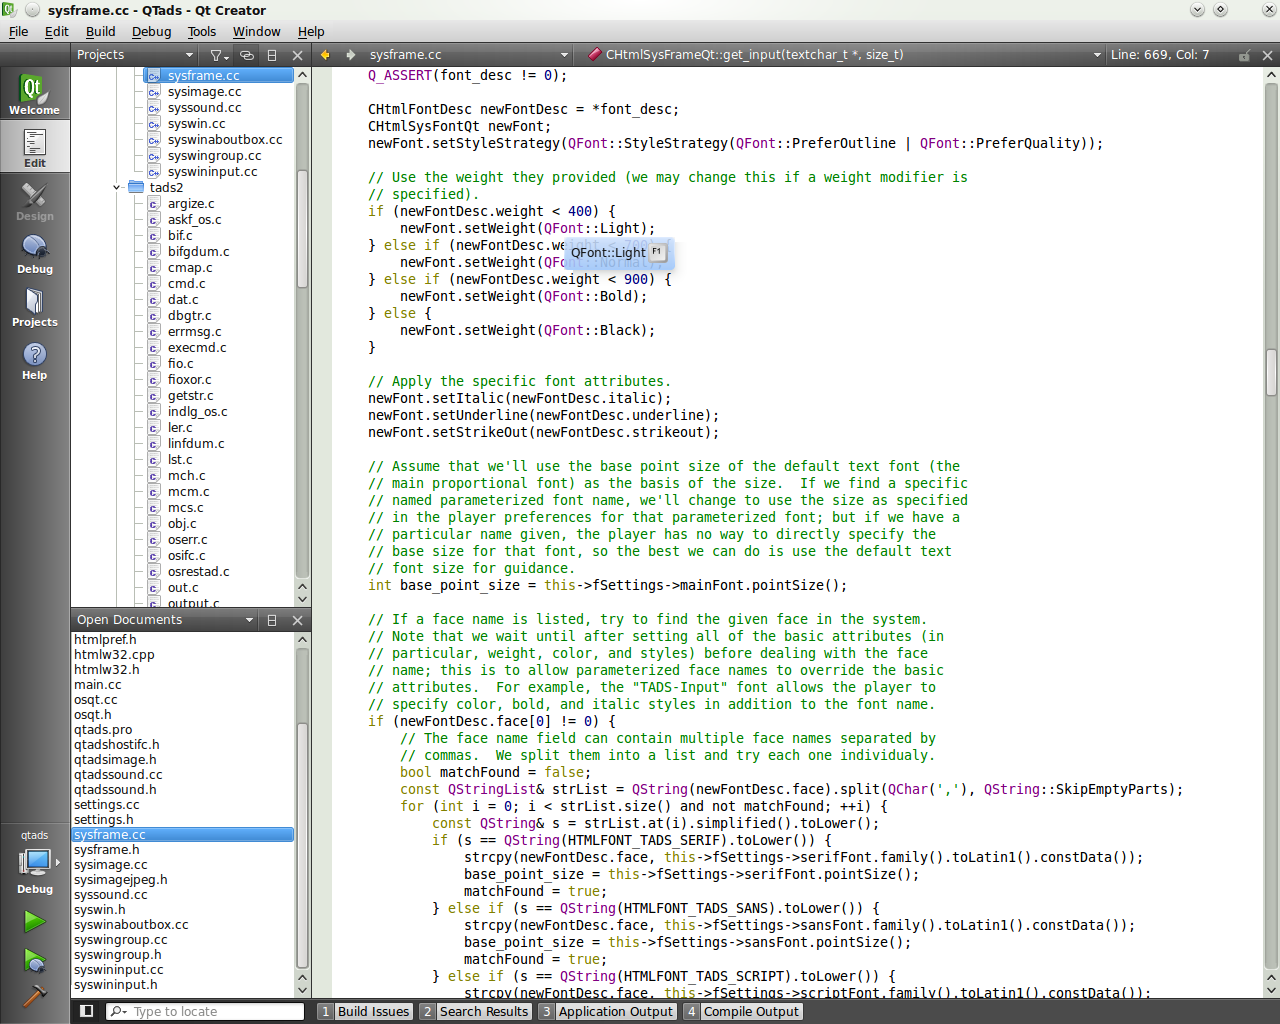
\includegraphics[width=\textwidth]{img/general/QtCreator.png}
\caption{QtCreator Version 2.0.1}
\label{QtCreator}
\end{center}
\end{figure}
\newpage
%Quellen:\\
%http://de.wikipedia.org/wiki/Qt_%28Bibliothek%29
%http://www.mathematik.uni-ulm.de/sai/ws02/cpp/070103/Qt.pdf
%http://wiki.ubuntuusers.de/Qt
%http://en.wikipedia.org/wiki/Qt_Creator


\section{Datenbank}
\label{section_Datenbank}

Für das Speichern der Messdaten und Betriebsparameter wird eine \ac{SQL} Datenbank verwendet. Bei der Wahl des Datenbankverwaltungssystems, standen mehrere Optionen zur Auswahl und die Entscheidung wurde zwischen SQLite und MySQL gefällt.
Beide System haben ihre Vor- und Nachteile.


\textbf{SQLite} ist ein \ac{SQL} Datenbankverwaltungssystem, welches ohne einen Server auskommt und operiert stattdessen in einer einzigen Datei. Es wird vor allem im Embedded Bereich eingesetzt, da kaum Konfigurationen oder Verwaltung notwendig ist. Deshalb eignet es sich ausgezeichnet für sich schnell weiterentwickelnde Applikationen.
\\
Aufgrund dieser Eigenschaften existieren allerdings auch Nachteile. So unterstützt SQLite nur eingeschränkt mehrere Nutzer gleichzeitig. Da das gesamte Datenbanksystem in einer einzigen Datei zusammengefasst ist, können mehrere zur selben Zeit durchgeführte Schreibzugriffe nicht unterstützt werden. Denn die einzige Sicherstellung der Datenintegrität erfolgt durch das Betriebssystem. 
\\
Des Weiteren ist SQLite aufgrund des Ein-Datei-Systems nur eingeschränkt skalierbar. Bei einer größeren Datenmenge oder erhöhten Anzahl an Zugriffen ist es nicht möglich diese Datei auf mehrere Systeme zu separieren, um somit die Last gleichmäßig zu verteilen.

\textbf{MySQL} ist ein weiteres \ac{SQL} Datenbankverwaltungssystem, welches allerdings auf einer Serverarchitektur beruht. 
Es ermöglicht die Verwaltung von Nutzern und Rechte. Außerdem ist das System gut hinsichtlich Performance und Größe zu skalieren. Zusätzlich bietet MySQL viele Möglichkeiten für Performanceanpassungen, wie z.B. Query-Caching.
\\
Jedoch gibt es auch hier Nachteile. So ist die Konfiguration wesentlich schwerer und komplexer. Durch die Notwendigkeit eines Servers benötigt MySQL mehr Ressourcen auf dem Host-System.

Die Wahl fällt auf das relationale Datenbankverwaltungssystem MySQL. Auch wenn SQLite einige Vorteile vor allem im Embedded Bereich besitzt, ist die fehlende Unterstützen von mehreren Nutzern gleichzeitig ein Ausschlusskriterium.

\cite{saake2010datenbanken}



\chapter{Anforderungsanalyse}
\label{chapter_Anforderungsanalyse}
Das Ziel dieser Arbeit ist es, einen Teststand zu entwickeln, der die Messung der Degradation von optoelektronischen Sendern ermöglicht. Dadurch soll eine Qualifizierung der Bauelemente erfolgen. In diesem Kapitel wird zunächst das Szenario näher beschrieben und anschließend die sich daraus entwickelnden Anforderungen definiert.

\section{Szenario}
Ein Unternehmen stellt verschiedene optoelektronischen Sensoren her. Zur Sicherstellung der Zuverlässigkeit der verwendeten \acp{LED} sollen diese mittels eines automatisierten Teststandes bezüglich ihres Degradationsverhaltens qualifiziert werden.


\begin{figure}[H]
\begin{center}
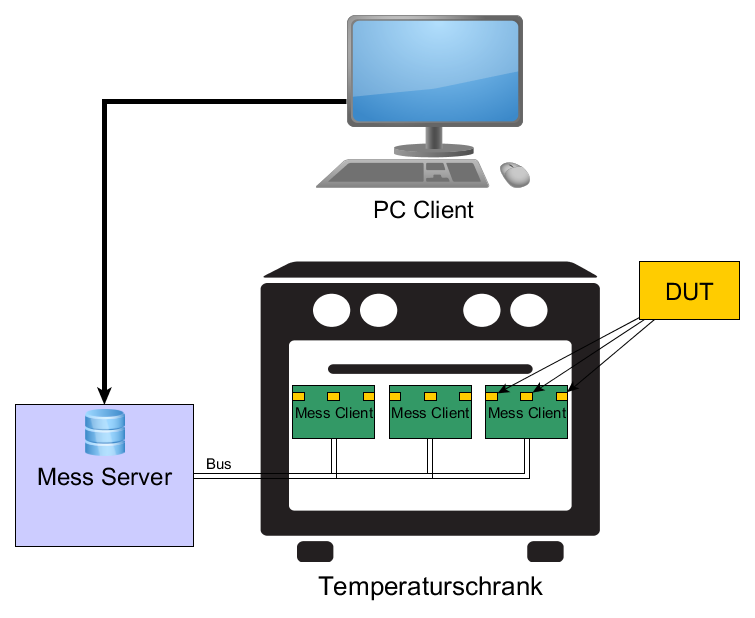
\includegraphics[width=0.6\textwidth]{img/general/Szenario.png}
\caption{Szenario}
\label{figure_Szenario}
\end{center}
\end{figure}

Der Teststand hat den in Abbildung \ref{figure_Szenario} zu sehenden Aufbau.
In einem Ofen befinden sich mehrere Mess-Clients. An diesen Mess-Clients sind jeweils 64 \acp{DUT} fest angeschlossen, bei denen das Degradationsverhalten aufgezeichnet werden soll.
Die Mess-Clients sind über einen Bus mit dem Mess-Server verbunden, welcher alle anfallenden Daten speichert.\\
Von einem PC-Client wird dann auf den Mess-Server zugegriffen um die Daten abzugreifen und grafisch auszuwerten.\\

\section{Analyse}

Die Akteure des Systems sind der Mess-Server, Mess-Client und PC-Client. Im Zuge dieser Arbeit soll der Mess-Server realisiert werden. Wobei die Interaktionsfähigkeit mit den anderen Akteuren sichergestellt werden muss.


\subsection{Mess-Client}
\label{section_Mess-Client}

Das Herzstück des Mess-Clients bildet ein STM8 8-Bit Mikrocontroller der Firma STMicroelectronics.
Auf jedem Mess-Client sind 64 \acp{DUT} befestigt. In zyklischen Abständen werden die Messdaten der Prüfobjekte aufgenommen und über eine RS232-Schnittstelle zur Verfügung gestellt.\\
Dieses System war zum großen Teil bereits gegeben, so dass lediglich die Übertragung der RS232 Schnittstelle geregelt werden musste. Dazu wurde ein Protokoll für die Kommunikation entworfen (sieht Abschnitt \ref{section_RS232_Protokoll}).
 
 \begin{figure}[!htb]
\minipage{0.48\textwidth}
  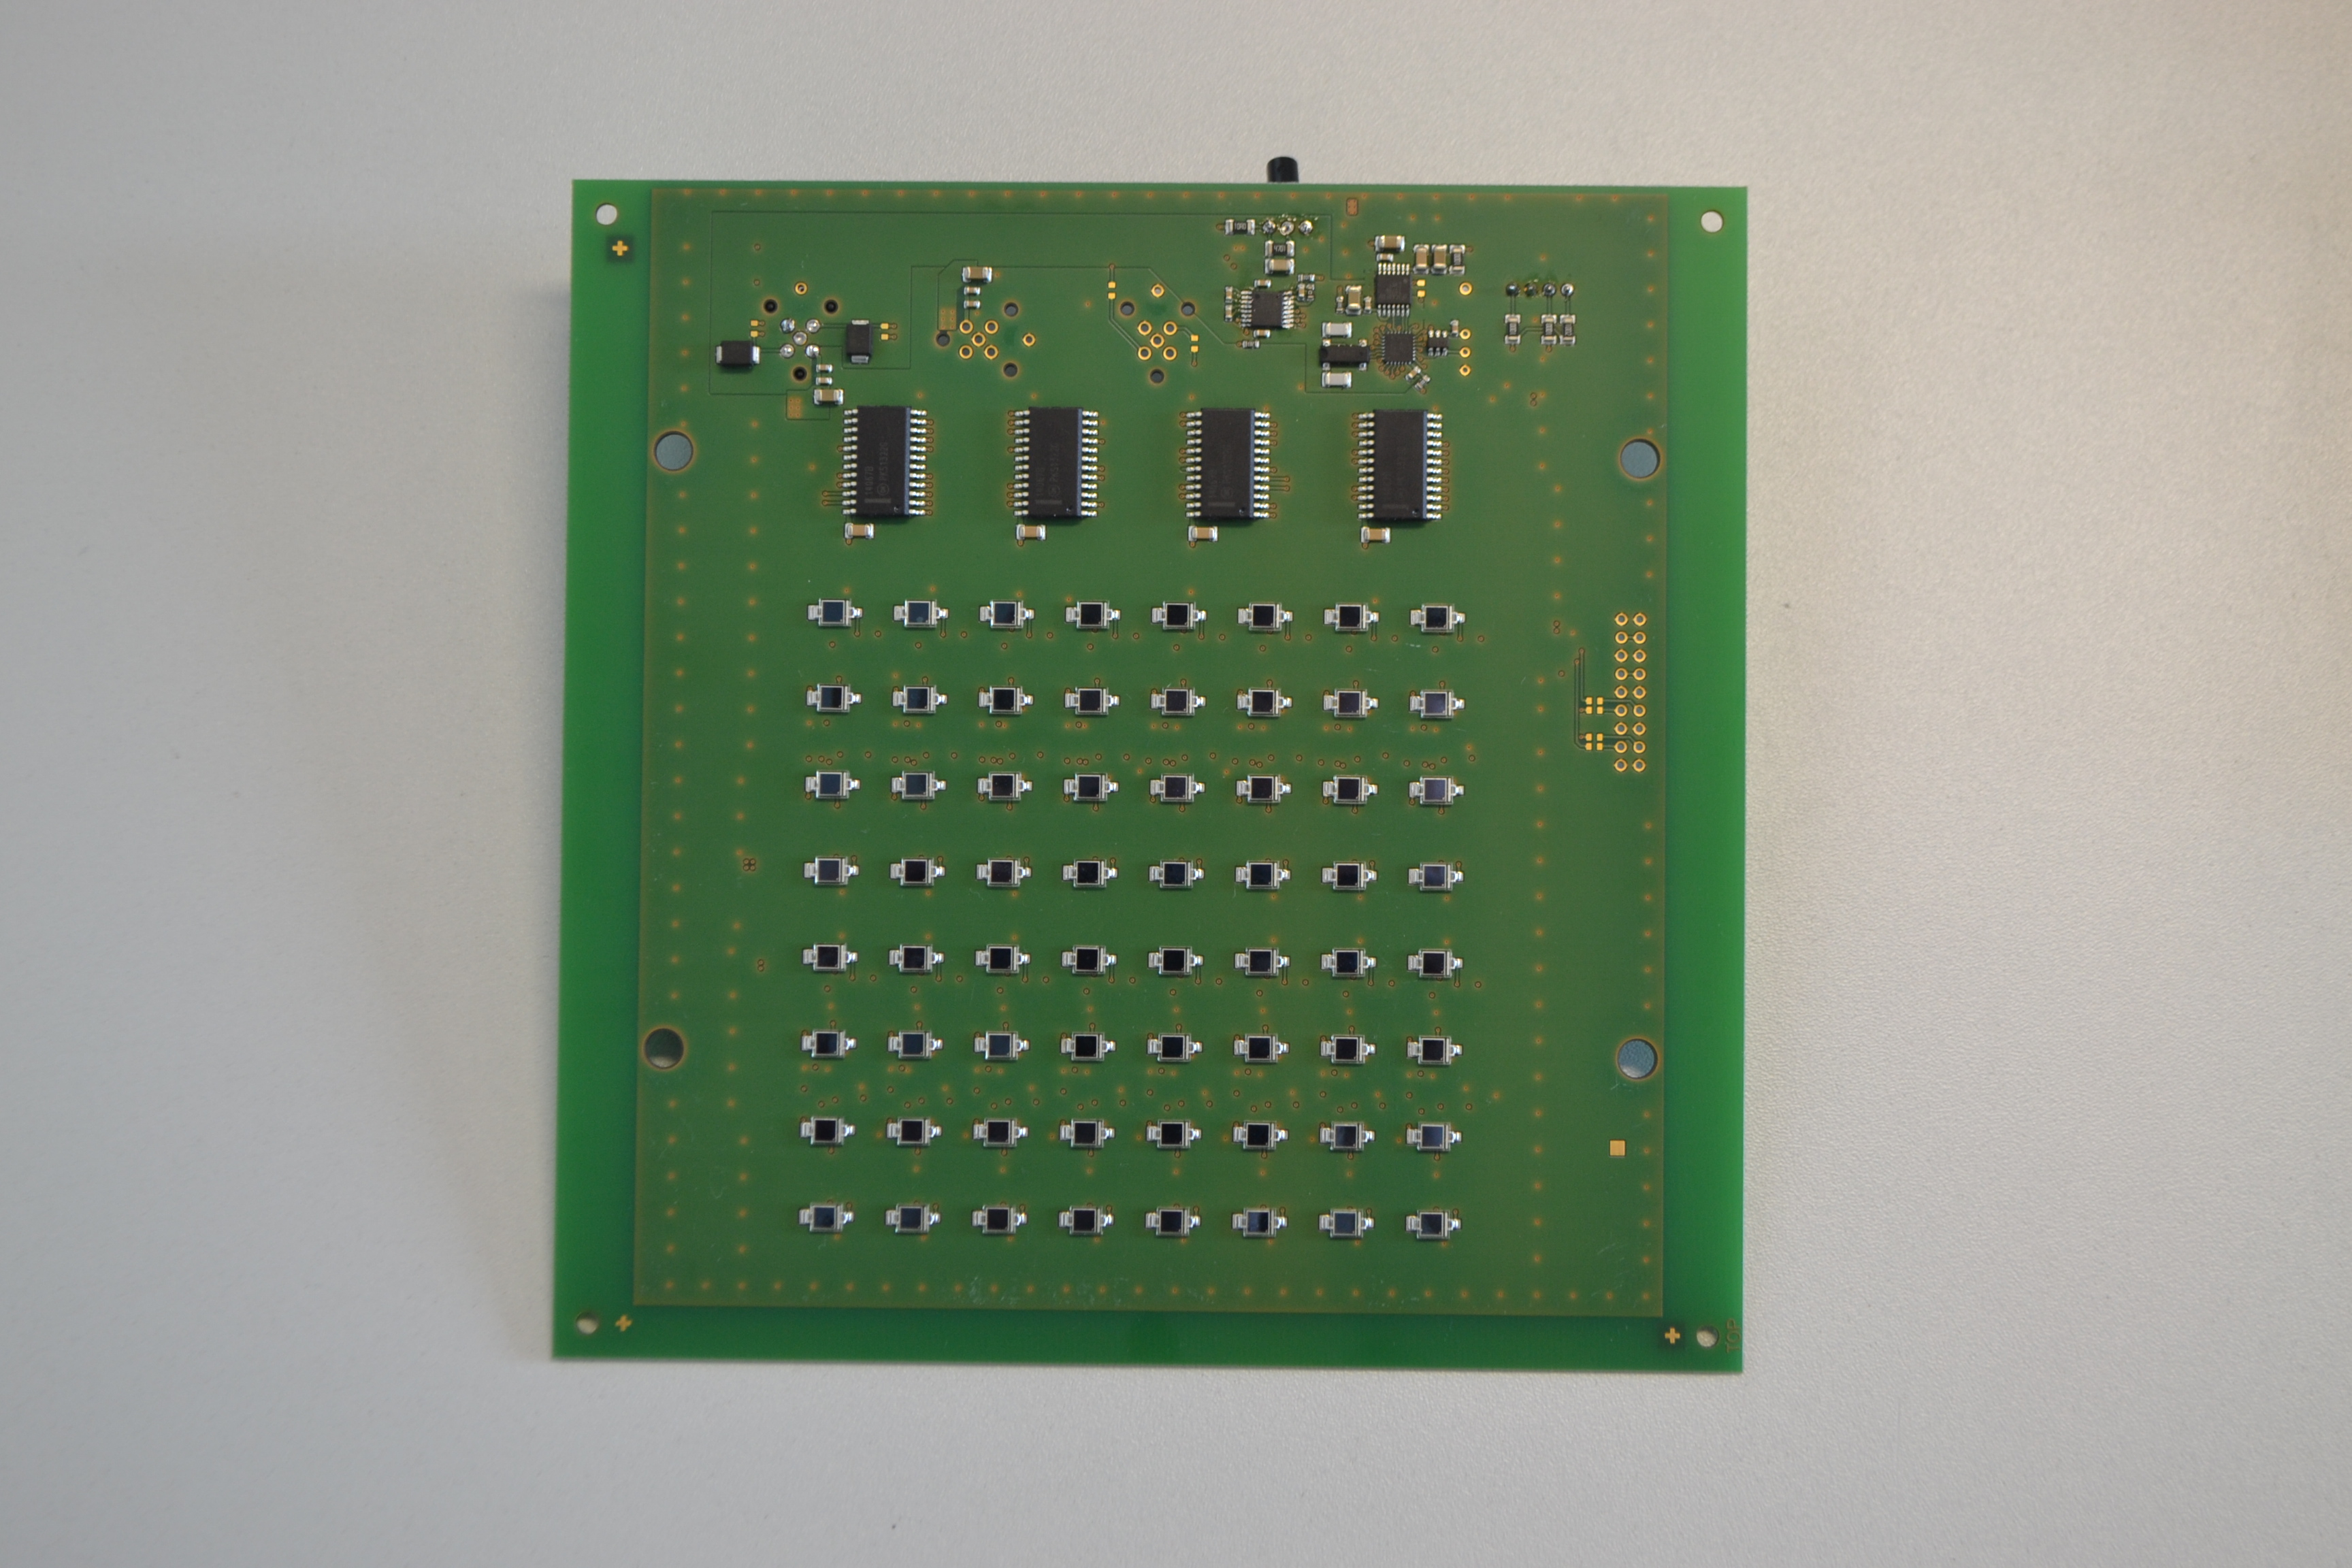
\includegraphics[width=\linewidth]{img/general/DegraBoardTop.jpg}
  \caption{Mess-Client Oberseite}\label{figure_DegraBoardTop}
\endminipage\hfill
\minipage{0.48\textwidth}%
  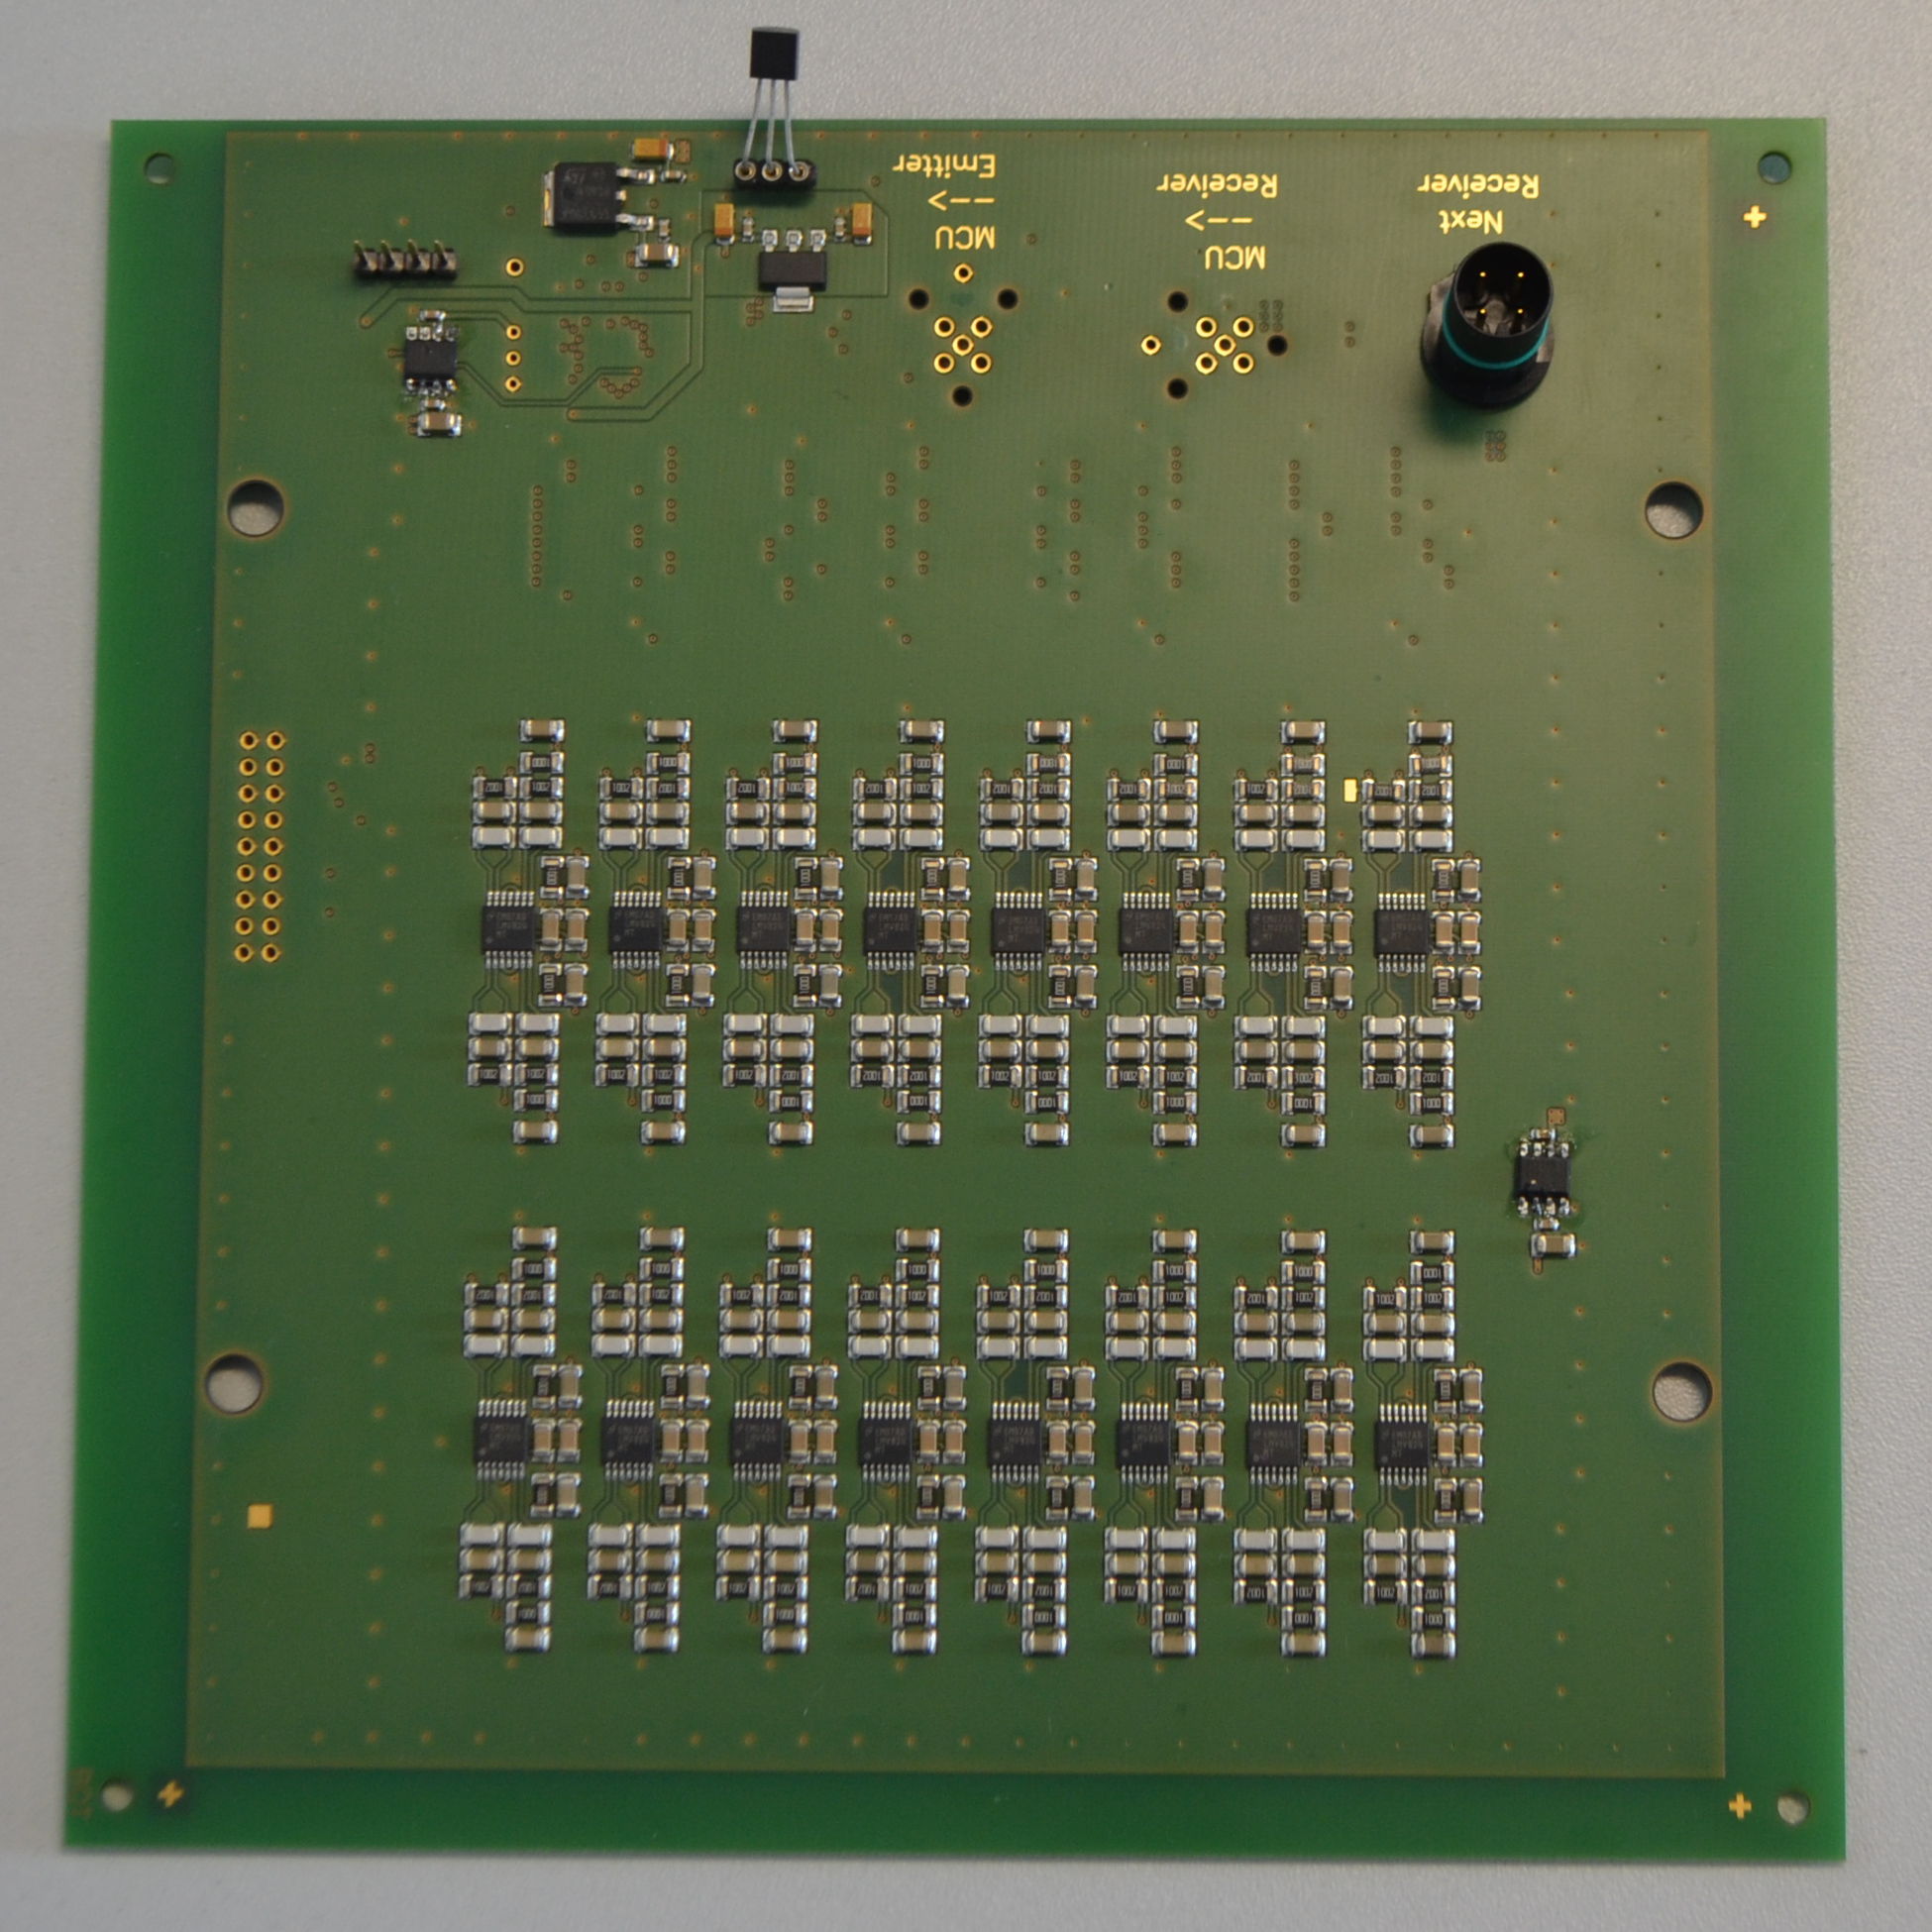
\includegraphics[width=\linewidth]{img/general/DegraBoardBottom.jpg}
  \caption{Mess-Client Unterseite}\label{figure_DegraBoardBottom}
\endminipage
\end{figure}


\textbf{------- Besondere RS232 chips, können RX hochohmig schalten. -------}


\subsection{Mess-Server}
\label{section_Mess-Server}

\begin{figure}[H]
\begin{center}
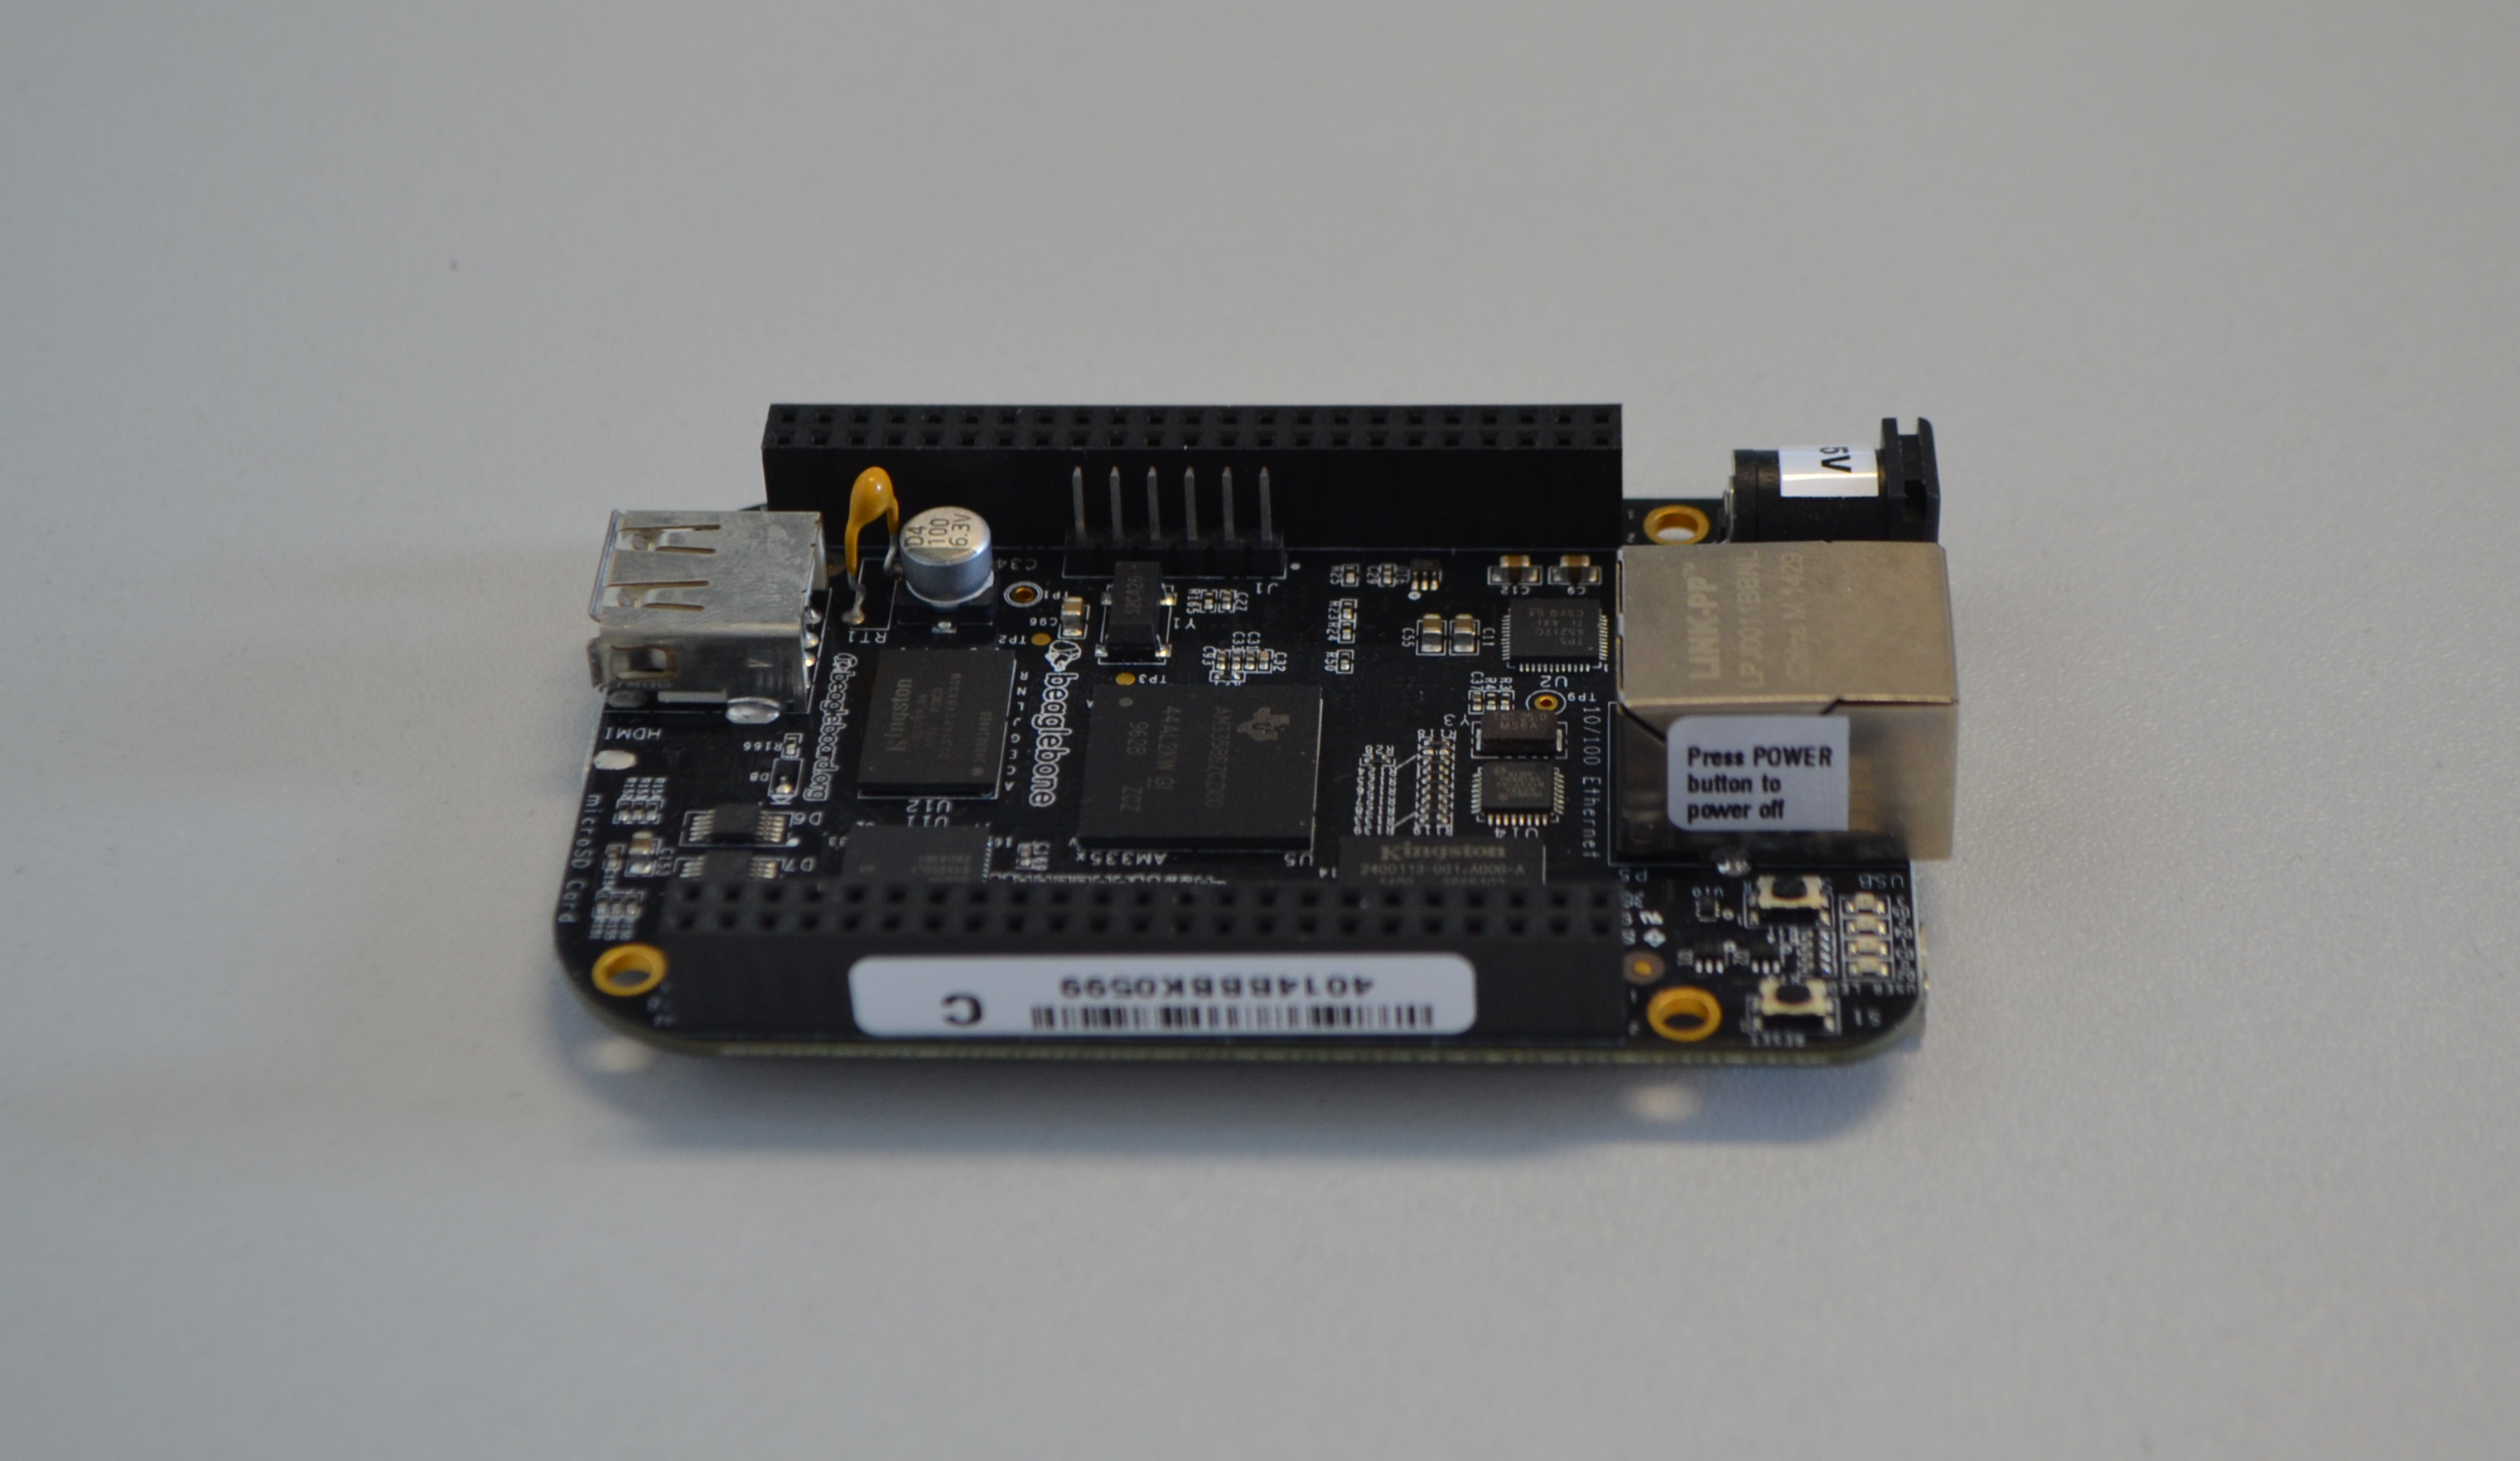
\includegraphics[width=0.6\textwidth]{img/general/BeagleBoneBlack.png}
\caption{BeagleBone Black}
\label{figure_Beagleboneblack}
\end{center}
\end{figure}


Als Mess-Server wird ein BeagleBone Black von Texas Instruments eingesetzt (siehe Abbildung \ref{figure_Beagleboneblack}). Dabei handelt es sich um einen kostengünstigen Einplatinencomputer mit offener Hardware. Damit ist es möglich, das BeagleBone Black auf individuelle Anforderungen anzupassen und selbst herzustellen. Auch gibt es eine große Community, die ständig die Entwicklung vorantreibt.
Die aktuelle Revision arbeitet mit einem AM335x 1GHz ARM® Cortex-A8 Prozessor, verfügt über 512MB DDR3 RAM und 4GB 8-bit eMMC internen Flash Speicher. Als Spannungsversorgung dient ein 5V 2A Netzteil.

Trotz der Kompaktheit des BeagleBone Black, bietet er ein ausreichendes Maß an Performance. Auf ihm kommt ein eingebettetes Debian-GNU/Linux Betriebssystem (sieht Abschnitt \ref{section_EmbeddedLinux}) zum Einsatz. \cite{schroeder2009embedded} sagt, dass es dadurch möglich ist die umfangreichen Linux-Funktionen wie die Paketverwaltung zu nutzen. Es biete auch den Vorteil, dass eine große Ähnlichkeit zu PC-Distributionen wie Ubuntu bestehe und somit die Linux Mechanismen einfach nutzbar seien. So kann das RS232 Interface beispielsweise wie eine normale Datei beschrieben und gelesen werden (sieht Abschnitt \ref{section_EmbeddedLinux}).

Für die Kommunikation mit den anderen Akteuren im System, muss ein RS232 Bussystem und eine Ethernet Schnittstelle realisiert werden. Des Weiteren soll ein MySQL Datenbankserver auf dem Mess-Server die effiziente Verwaltung von Daten übernehmen.

\subsection{PC-Client}
\label{section_PC-Client}
Der PC-Client stellt eine Qt Desktopanwendung mit \ac{GUI} zur Auswertung der Messdaten dar. Über das Netzwerk ruft er die Messdaten von dem Mess-Server ab. 


\section{Anforderungen}

Folgende Anforderungen werden dabei an das System gestellt:
\begin{itemize}
\item Individuelle Parametrierung der \acp{DUT}
\item Automatische Erfassung der Messdaten
\item Fernzugriff auf den Mess-Server
\end{itemize}
\ \\
\textbf{Individuelle Parametrierung der \acp{DUT}}\\
Immer 64 \acp{DUT} befinden sich auf einem Mess-Client. Dabei sollen verschiedene Parameter für die \acp{DUT} berücksichtigt werden. 
Zum einen sollen die Intervalle in denen Messwerte aufgenommen werden konfigurierbar sein. Dies soll in mindestens 3 verschiedenen Intervallen möglich sein.

Beispiel: 

\begin{table}[H]
\begin{center}
\begin{tabular}{|l|l|}\hline
Zeitraum & Zeit zwischen Messungen \\ \hline
1. Woche & 12 Stunden\\ 
2. bis 4. Woche & 2 Tage\\ 

ab 5. Woche & 7 Tage\\ \hline
\end{tabular}
\caption{Intervalle}
\label{table_Intervalle}
\end{center}
\end{table}



Des Weiteren soll für jeden Mess-Client ein Pulsepattern definierbar sein. Dieses Pulsepattern wird dann als Versorgungssignal für die \acp{DUT} verwendet.

\textbf{Automatische Erfassung der Messdaten}\\
Die Messdaten der \acp{DUT} sollen zyklisch erfasst werden. Es soll die derzeitige Temperatur im Ofen, der gemessene Wert des Sensors und ein Zeitstempel gespeichert werden. Dabei sollen, wie bereits erwähnt, die Intervalle zwischen den Messungen konfigurierbar sein.\\
Für den einfachen und effizienten Zugriff auf die Daten, sollen diese in einer \ac{SQL} Datenbank abgelegt werden. Dafür ist eine Kommunikationsschnittstelle zwischen der Datenbank und den Mess-Clients erforderlich, welcher über den Mess-Server realisiert werden soll.

\textbf{Fernzugriff auf den Mess-Server}\\
Zur Auswertung der Messdaten, soll es möglich sein, von einem PC-Arbeitsplatz aus eine Verbindung zu dem Mess-Server aufzubauen. Die Messdaten sollen dann grafisch auf dem PC-Client zur Auswertung aufbereitet werden.
Auch soll ein Tunnelmodus direkten Zugriff von einem PC-Client auf einem Mess-Client ermöglichen. Dabei sollen die Parameter des Mess-Clients verändert werden können.


Diese Basis-Anforderungen und einige zusätzliche Anforderungen können wie in Tabelle \ref{table_Anforderungen} in funktionale und nicht-funktionale Anforderungen unterteilt werden.


\begin{table}[H]
\begin{center}
\begin{tabularx}{\textwidth}{|p{3cm}|X|X|X|}\hline
Art & Anforderung & Kommentar \\ \hline
Nicht-Funktional & Das System soll jederzeit verfügbar sein. & Bei Fehlern soll das System ohne große Ausfallzeit wieder Einsatzbereit sein. Zuverlässigkeit ist sehr wichtig.\\ \hline
Nicht-Funktional & Das Benutzerinterface soll zeitnah auf Anfragen reagieren. & Um Benutzerfreundlichkeit zu gewährleisten, soll auf Nutzeranfragen ohne lange Wartezeiten reagiert werden. \\ \hline
Funktional & Das System soll das Degradationsverhalten eines \ac{DUT} aufnehmen & Hauptanforderung des Systems. Messdaten sollen zu einem \ac{DUT} gesammelt werden, um den Grad der Degradation bestimmen zu können. \\ \hline
Funktional & Neue Mess-Clients sollen am PC-Client parametrierbar sein. & Parameter sollen auf dem Mess-Client und in einer Datenbank gespeichert werden. \\ \hline
Funktional & Neue bereits parametrierte Mess-Clients sollen automatisch in das System integrierbar sein. & Ein parametrierter Mess-Client kann direkt an den Bus im Ofen angeschlossen werden.\\ \hline
Funktional & Zyklische Erfassung von Messdaten. & Intervalle der Messdatenerfassung sind konfigurierbar.\\ \hline
Funktional & Messdaten sollen grafisch dargestellt werden. & Um die Daten auswerten zu können sollen sie grafisch aufbereitet werden.\\ \hline
Funktional & Die Messdaten sollen in einer Datenbank abgelegt werden. & Zum einfachen und effizienten Zugriff auf die Daten.\\ \hline
Funktional & Die Messdaten sollen via Fernzugriff erreichbar sein. & Von einem PC-Client aus, soll auf die Daten im lokalen Netzwerk zugegriffen werden können.\\ \hline
Funktional & Der Status des Systems soll ablesbar sein. & Über eine Anzeige soll das System lokal überwacht werden können.\\ \hline
Funktional & Nutzer Fehler sollen abgefangen werden. & Fehler bei der Bedienung durch den Nutzer sollen unterbunden werden.\\ \hline
\end{tabularx}
\caption{Anforderungen}
\label{table_Anforderungen}
\end{center}
\end{table}














\chapter{Design}
\label{chapter_Design}

Im folgenden Kapitel wird auf das Design des Systems eingegangen. Zunächst wird auf den Aufbau der Hardware eingegangen. Anschließend wird sich näher mit dem Design und dem Aufbau der einzelnen Softwareelemente befasst. Zum Ende des Kapitels gibt es einen genaueren Einblick in die Gestaltung und den Aufbau des Protokoll für die RS232 Schnittstelle.

\section{Übersicht}
\label{section_Teststand}

Das Gesamtsystem setzt sich aus drei Akteuren zusammen. Der folgenden Abschnitt gibt eine kurze Übersicht über die Hauptaufgaben der einzelnen Systeme.

\begin{itemize}

\item Mess-Server
\begin{itemize}
\item Verwaltet angeschlossene Mess-Clients.
\item Speichert alle Messdaten in einer Datenbank.
\item Ermöglicht den Fernzugriff von einem PC-Client.
\end{itemize}

\item Mess-Client
\begin{itemize}
\item Übernimmt die lokale Ansteuerung der \acp{DUT}.
\item Nimmt Messdaten auf und stellt sie zur Verfügung.
\end{itemize}

\item PC-Client
\begin{itemize}
\item Parametriert die Mess-Clients.
\item Wertet Messdaten aus und stellt sie leserlich da.
\end{itemize}

\end{itemize}


\begin{figure}[H]
\begin{center}
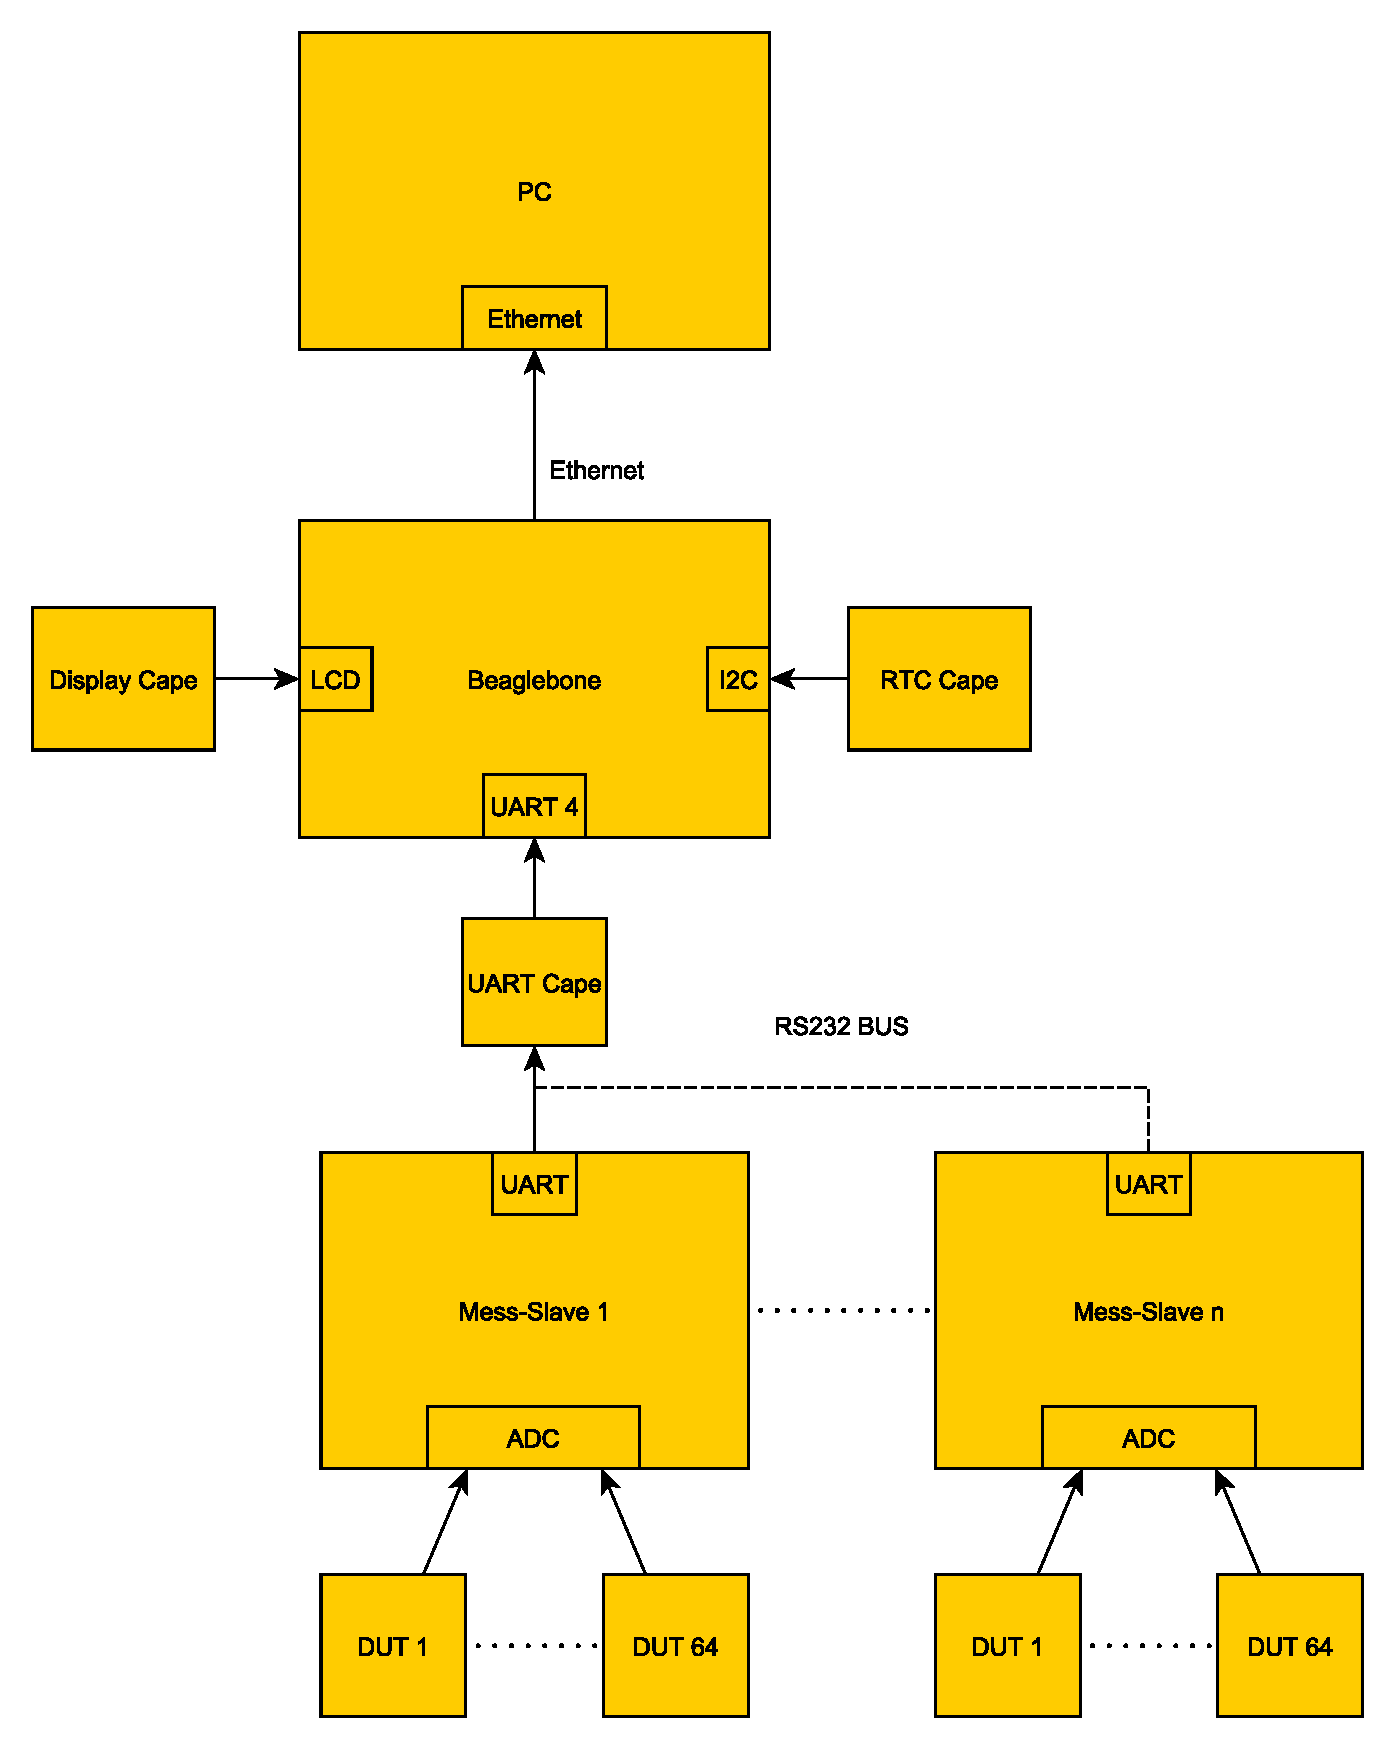
\includegraphics[width=\textwidth ]{img/general/BlockPlan.pdf}
\caption{Übersicht}
\label{figure_Übersicht}
\end{center}
\end{figure}


\section{Mess-Server}
\label{section_Mess-Server}

Als Mess-Server wird ein BeagleBone Black von Texas Instruments eingesetzt. Dabei handelt es sich um einen kostengünstigen Einplatinencomputer mit offener Hardware. Damit ist es möglich, das BeagleBone Black auf individuelle Anforderungen anzupassen und selbst herzustellen. Auch gibt es eine große Community, die ständig die Entwicklung vorantreibt.
Er arbeitet mit einem AM335x 1GHz ARM® Cortex-A8 Prozessor, verfügt über 512MB DDR3 RAM und 4GB 8-bit eMMC internen Flash Speicher. Als Spannungsversorgung dient ein 5V 2A Netzteil.


\begin{figure}[H]
\begin{center}
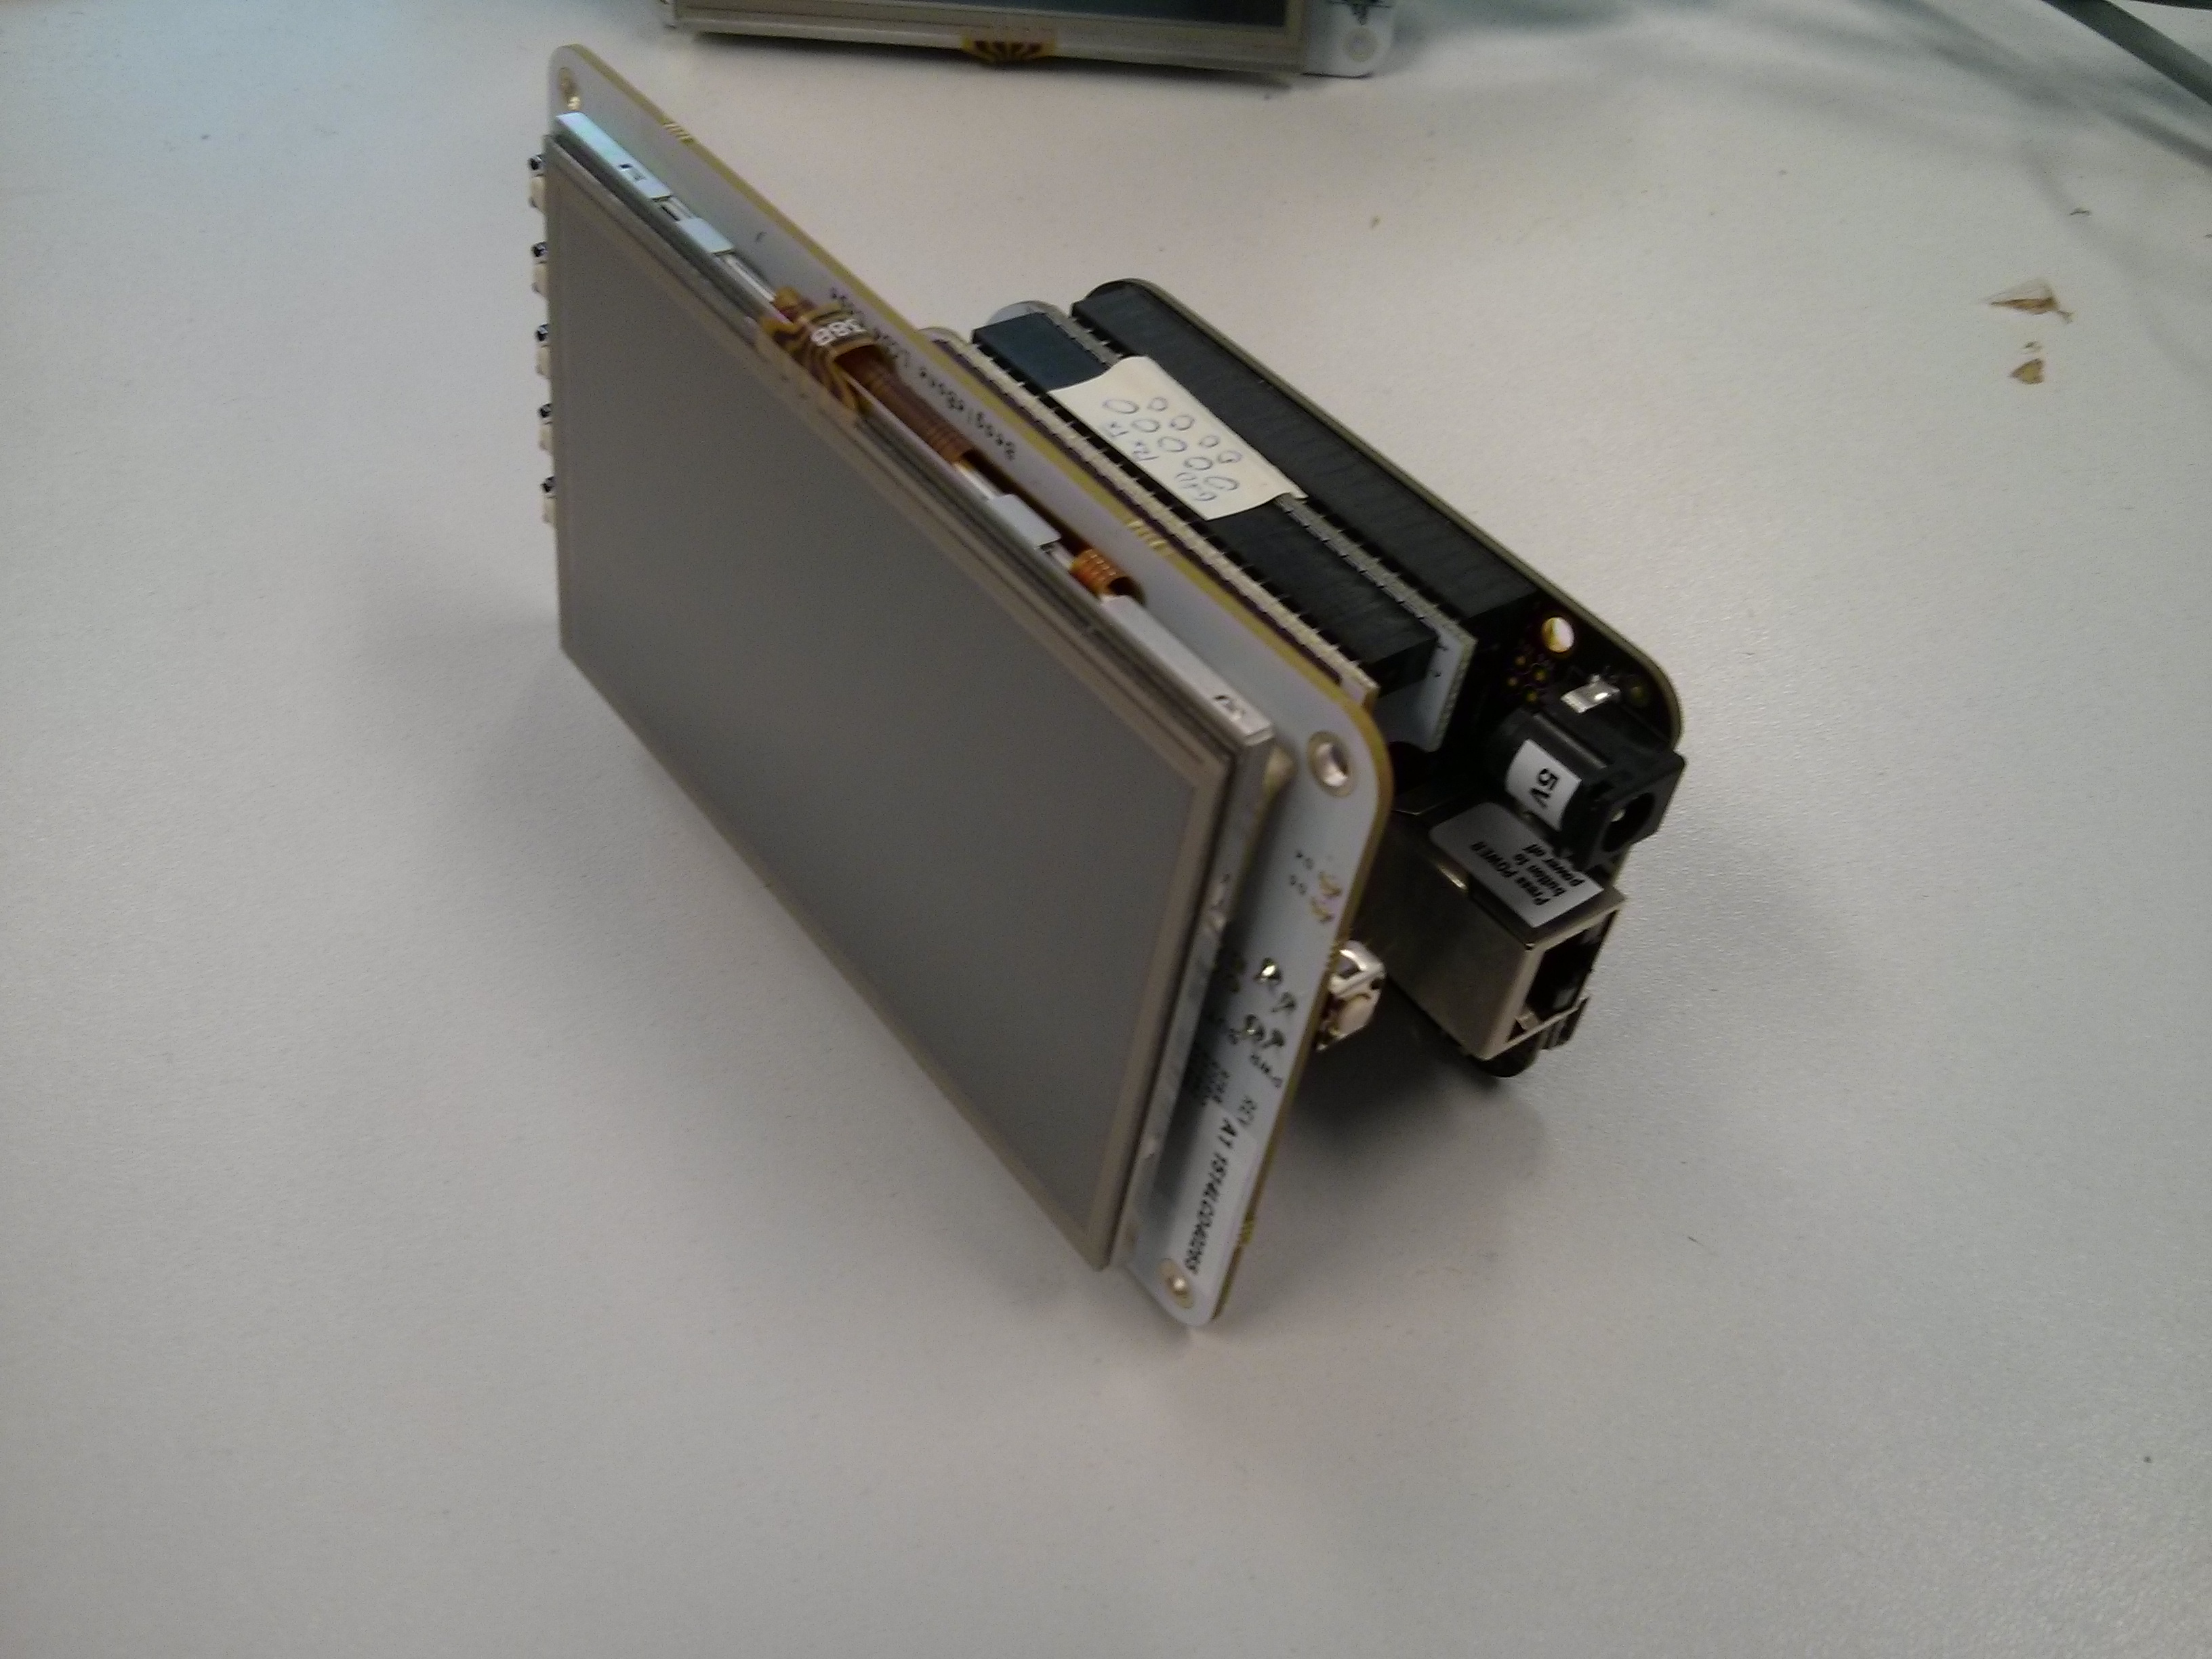
\includegraphics[width=0.8\textwidth]{img/general/BeagleBoneBlack.jpg}
\caption{BeagleBone Black}
\label{figure_Beagleboneblack}
\end{center}
\end{figure}

Trotz der Kompaktheit des BeagleBone Black, bietet er ein ausreichendes Maß an Performance. Auf ihm kommt ein Debian-GNU/Linux Betriebssystem zum Einsatz. Damit ist es möglich die umfangreichen Debian-Funktionen wie die Paketverwaltung zu nutzen. Es bietet auch den Vorteil, dass eine große Ähnlichkeit zu PC-Distributionen wie Ubuntu besteht und somit einfacher nutzbar ist (vgl. \cite{schroeder2009embedded}).\\
Außerdem sind Linux Mechanismen einfach nutzbar. So kann das RS232 Interface beispielsweise wie eine normale Datei beschrieben und gelesen werden.

\subsection{Hardware}
\label{ServerHardware}

\begin{figure}[H]
\begin{center}
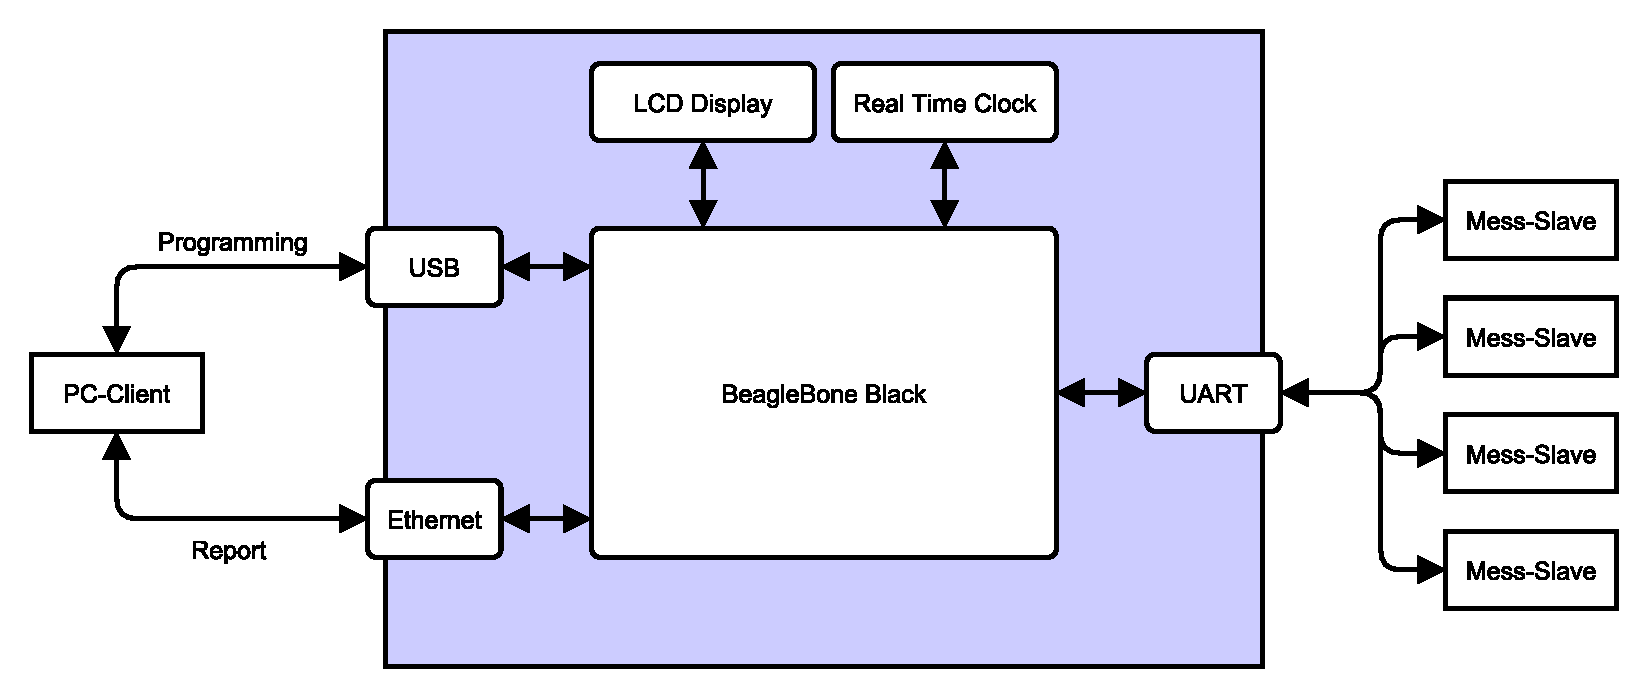
\includegraphics[width=\textwidth ]{img/general/UebersichtMaster.pdf}
\caption{Aufbau Mess-Server}
\label{figure_AufbauBleagleBone}
\end{center}
\end{figure}

Das BeagleBone selbst ist bereits sehr Leistungsstark. Um jedoch weiter Funktionen und Schnittstellen hinzuzufügen, existieren Capes. Ein Cape ist eine für das BeagleBone konzipierte Erweiterung, die direkt auf das BeagleBone aufgesteckt werden kann. Die Treiber vieler dieser Capes sind bereits in dem Betriebssystem des BeagleBones integriert oder werden vom Hersteller bereitgestellt. Somit ist die Inbetriebnahme sehr komfortable.


\textbf{ABBILDUNG EINES CAPES}


Zur Kommunikation mit den Mess-Clients wird die \ac{UART} Schnittstelle des BeagleBone Black verwendet. Dafür wird ein RS232 Cape eingesetzt. Das Cape führt die seriellen Ports UART0, UART1, UART2 und UART4 auf einen 9-poligen seriellen Stecker. Es bietet die Möglichkeit zwischen den verschiedenen Ports mittels eines Jumper auf dem Cape zu wechseln. Angeschlossen wird nach dem 3-wire Prinzip. Dabei werden lediglich Rx, Tx und die Masse verbunden. Somit ist keine Hardware-Flusssteuerung möglich.\ 

Da das BeagleBone Black kein eigenes \ac{RTC} Modul besitzt, wird auch dieses durch ein Cape hinzugefügt. Es beinhaltet eine 3V Knopfbatterie um auch im Falle einer Stromunterbrechung die aktuelle Zeit nicht zu verlieren. Dies ist sehr wichtig, da es erforderlich ist, dass das BeagleBone die aktuelle Uhrzeit und das aktuelle Datum jederzeit kennt. Denn beim Erfassen der Messdaten wird ein Zeitstempel angelegt um die Daten später zeitlich zuordnen zu können. Sollte dieser Zeitstempel nicht korrekt sein, sind die Daten bei der Auswertung nicht gültig.\ 

Um die Statusanzeige detailliert darstellen zu können, wird ein resistives LCD-Touchscreen Display eingesetzt. Es hat eine Größe von 4,3 Zoll bei einer Auflösung von 480x272 Pixeln. Dabei handelt es sich ebenso um ein Cape. Dadurch ist es möglich, das BeagleBone Black trotz den Erweiterungen kompakt zu halten. Denn die Capes sind untereinander Stapelbar.\ 


\textbf{ABBILDUNG gestapeltes BeagleBone}


Die USB Schnittstelle, welche zur Programmierung des BeagleBones verwendet wird, ist bereits vollständig einsatzbereit. Ebenso ist die Ethernet Schnittstelle, welche für den Fernzugriff auf das BeagleBone genutzt wird, bereits standardmäßig vollständig integriert.

\subsection{Software}
\label{ServerSoftware}
Die Programmierung der Software erfolgt in C++ unter Verwendung der Klassenbibliothek Qt (siehe Abschnitt \ref{section_Qt}).\\
Das Softwaredesign teilt sich in einen sequentiellen Teil für die Abfrage und Speicherung der Messwerte, sowie einen Event gesteuerten Teil für die \ac{GUI} und die externe Kommunikation für die Fernzugriffe. Die beiden Programmteile können unabhängig von einander agieren und kommunizieren ausschließlich über Signale und Slots (siehe \ref{QtSignaleSlots}). Durch diese Kapselung ist es möglich die beiden Programmteile durch andere Lösungen auszutauschen, welche lediglich die selben Signale und Slots unterstützen müssen.\ 

\subsubsection{Messdatenerfassung}
Der Hauptzyklus der Software ruft kontinuierlich die Messdaten von den Mess-Clients ab. Dafür wird ständig geprüft ob Messungen erforderlich sind. Dies geschieht durch den Vergleich der vergangenen Zeit zur letzten Messung und den gegebenen Parametern für die Messintervalle. In der Tabelle \ref{table_ParameterMessintervalle} finden sich diese Parameter.\\


\begin{table}[H]
\begin{center}
\begin{tabular}{|l|l|}\hline
Parameter & Beschreibung \\ \hline
duration\_int1 & Dauer der Zeit die Werte im 1.Interval aufgenommen werden in Tagen\\  \hline
duration\_int2 & Dauer der Zeit die Werte im 2.Interval aufgenommen werden in Tagen\\  \hline
interval\_1 & Abstand zwischen den Messungen im 1. Interval in Minuten\\  \hline
interval\_2 & Abstand zwischen den Messungen im 2. Interval in Minuten\\  \hline
interval\_3 & Abstand zwischen den Messungen nach dem 2. Interval in Minuten\\ \hline
\end{tabular}
\caption{Parameter der Messintervalle}
\label{table_ParameterMessintervalle}
\end{center}
\end{table}


Ob eine Messung erforderlich ist, lässt sich aus den gegebenen Parametern ableiten. So wird zuerst geprüft, welcher Zeitraum (\textit{duration\_int1-2}) derzeit zutrifft. Dazu wird die vergangene Zeit seit der ersten Messung mit dem Zeitraum abgeglichen. Sollten noch keine Ergebnisse vorhanden sein, ergibt dies die Erforderlichkeit einer Messung. Wenn der passende Zeitraum ausgemacht ist, wird das dazugehörige Intervall zwischen den einzelnen Messungen (\textit{interval\_1-3}) ausgemacht. Dann wird geprüft, ob die vergangene Zeit seit der letzten Messung größer ist als dieses Intervall.\ 

Anschließend wird geprüft ob der Mess-Client verfügbar ist. Dazu wird eine Namensanfrage über die RS232 Schnittstelle verschickt. Bei einer positiven Antwort wird dann eine Messung durchgeführt. Dabei werden alle \acp{ADC} der 64 möglichen \acp{DUT} mittels \textit{ADC-Value}-Befehls (siehe Tabelle \ref{table_Commands}) ausgelesen. Sobald alle 64 Werte erfolgreich ermittelt sind, werden sie in der Datenbank abgelegt. \\
Sollte keine Antwort auf die Namensanfrage erfolgen, wird in den nächsten Zyklen erneut versucht eine Verbindung zu etablieren. Bei kontinuierlich erfolglosen Verbindungsversuchen, informiert das System den Nutzer nach einer festgelegten Zeit der Abwesenheit über die Unerreichbarkeit.
 
\begin{figure}[H]
\begin{center}
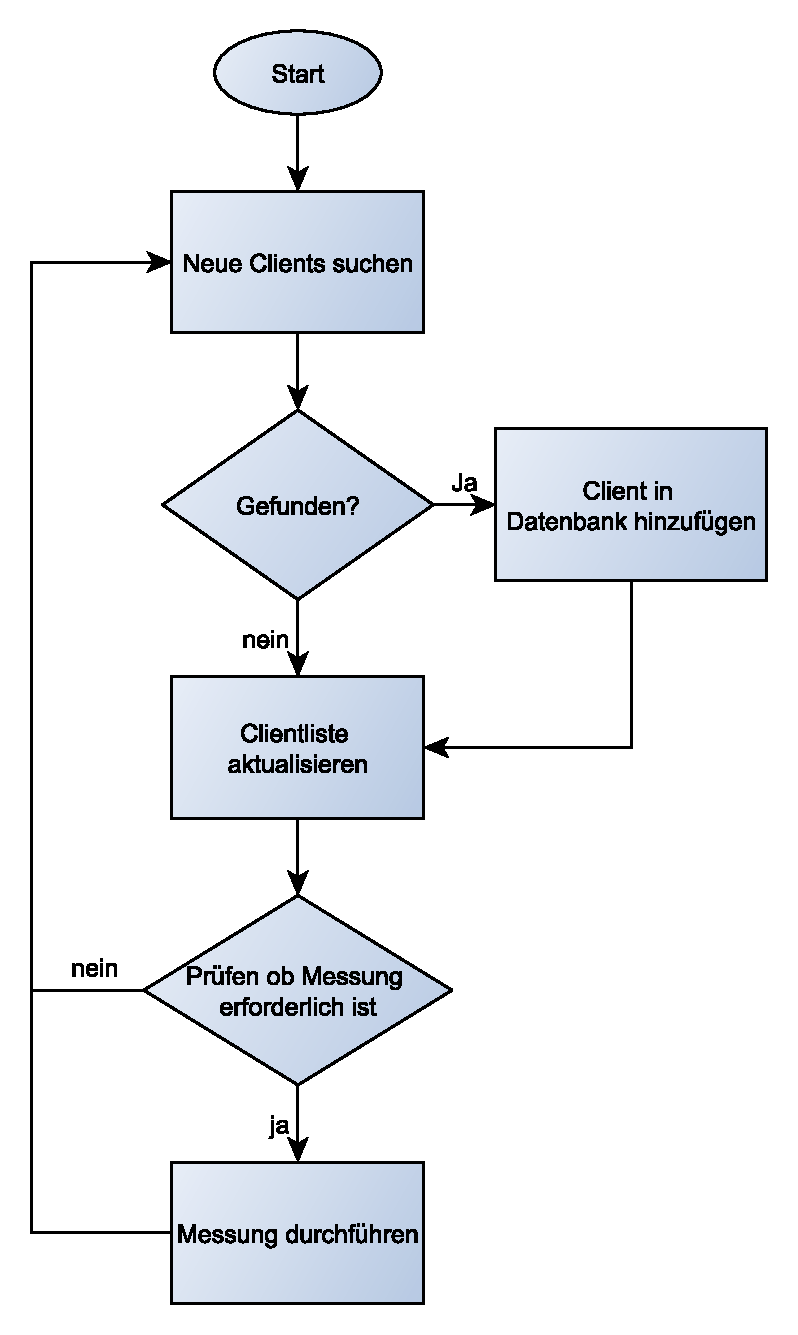
\includegraphics[width=0.5\textwidth ]{img/general/Ablaufplan_Master.pdf}
\caption{Ablaufplan}
\label{figure_Ablaufplan_Master}
\end{center}
\end{figure}
 
\newpage
\subsubsection{Benutzeroberfläche}
Um die Anforderung der Statusüberwachnung zu erfüllen, verfügt das BeagleBone über eine \ac{GUI}. Sie bietet einen einfachen Überblick über die aktuellen Vorgänge und soll auf einen Blick den Status des Mess-Servers wiedergeben.\\
Am oberen Rand der \ac{GUI} (sieht u.a. Abbildung \ref{figure_MessServerGUIStatus}) wird das aktuelle Datum und die aktuelle Uhrzeit angezeigt, sowie die derzeitige IP Adresse und der aktuelle Name. Am unteren Rand wird die derzeit ausführende Aktion in einer Statusnachricht ausgegeben.
Die \ac{GUI} ist dabei in vier Tabs unterteilt.

\textbf{Status Tab}

\begin{figure}[H]
\begin{center}
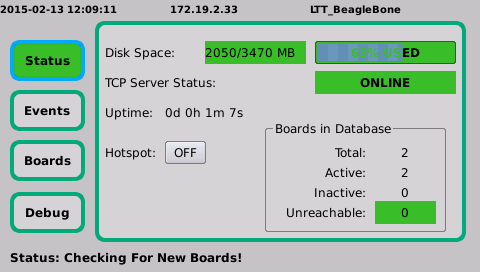
\includegraphics[width=0.5\textwidth ]{img/GUI/Server_GUI_Status1.png}
\caption{Mess-Server GUI: Status Tab}
\label{figure_MessServerGUIStatus}
\end{center}
\end{figure}

Das Erste ist das Status-Tab (siehe Abbildung \ref{figure_MessServerGUIStatus}). Es zeigt die wichtigsten Statusdaten wie verfügbarer Speicher, die aktuelle Laufzeit und TCP Server Status an. Um auf einen Blick den Status des Systems zu erkennen wird mittels der Farben grün und rot ein positiver bzw. negativer Status signalisiert.

\textbf{Events Tab}

\begin{figure}[H]
\begin{center}
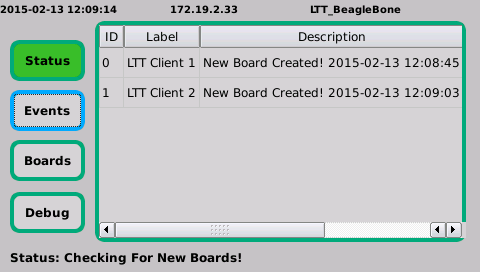
\includegraphics[width=0.5\textwidth ]{img/GUI/Server_GUI_Events1.png}
\caption{Mess-Server GUI: Events Tab}
\label{figure_MessServerGUIEvents}
\end{center}
\end{figure}

Im Events Tab werden wichtige Ereignisse dargestellt. 

\textbf{Boards Tab}

\begin{figure}[H]
\begin{center}
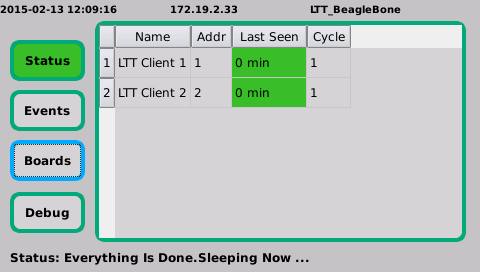
\includegraphics[width=0.5\textwidth ]{img/GUI/Server_GUI_Boards1.png}
\caption{Mess-Server GUI: Boards Tab}
\label{figure_MessServerGUIBoards}
\end{center}
\end{figure}

Das Boards Tab zeigt die derzeit aktiven Mess-Clients in einer Liste an. Als aktiv werden Mess-Clients bezeichnet, die mit einer gültigen Adresse in der Datenbank eingetragen sind. Angezeigt werden der Name, die Adresse, die vergangene Zeit seit dem es das letzten mal erfolgreich kontaktiert wurde und die Anzahl der erfolgreichen aufgenommenen Messzyklen.

\textbf{Debug Tab}

\begin{figure}[H]
\begin{center}
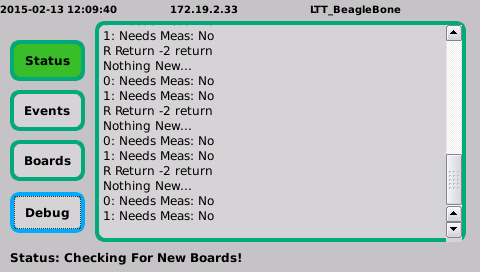
\includegraphics[width=0.5\textwidth ]{img/GUI/Server_GUI_Debug2.png}
\caption{Mess-Server GUI: Debug Tab}
\label{figure_MessServerGUIDebug}
\end{center}
\end{figure}

Der Zweck des Debug Tabs ist es die im Programmcode erzeugten Nachrichten anzuzeigen. Somit soll es möglich sein Fehler einfacher zu erkennen.

\subsubsection{RS232 Kommunikation}
Die RS232 Schnittstelle wird ausschließlich zur Kommunikation mit den Mess-Clients verwendet. Um die Erfolgschancen der Anfragen zu erhöhen, werden Fehlschläge erkannt und durch den Versuch des erneuten Sendens minimiert. Zwischen jedem Sendeversuch befindet sich eine kurze Verzögerung.
 

\subsubsection{Ethernet Kommunikation}

Um auf Netzwerkanfragen reagieren zu können, ist sowohl ein UDP-Server für Broadcast-Nachrichten als auch ein TCP-Server für die direkte Kommunikation realisiert.\\
Der UDP-Server dient dabei zur dynamischen Erkennung im Netzwerk. Dabei antwortet der Mess-Server auf Broadcast-Nachrichten mit seiner IP-Adresse und seinem Namen. Dies ermöglicht die einfache Eingliederung der Mess-Server in ein Netzwerk.
Der TCP-Server nimmt RS232- und SQL-Befehle an und leitet diese weiter. Dies ermöglicht den Fernzugriff auf die einzelnen Mess-Clients über ein Netzwerk. 

\begin{table}[H]
\begin{center}
\begin{tabularx}{\textwidth}{|c|c|c|X|}\hline 
 Command & Typ & Daten & Kommentar \\ \hline
 BeagleSendYourIP & UDP & - & Das BeagleBone antwortet dem Sender mit seiner IP Adresse und seinem Namen  \\ \hline
 BeagleUpdateConfig & UDP & - & Das BeagleBone aktualisiert seine Konfiguration aus der Config-Datei \\ \hline
 RS232CMD: & TCP & RS232 Rahmen & Das BeagleBone sende den empfangenen Rahmen über seine RS232 Schnittstelle \\ \hline
 SQLCMD: & TCP & SQL Anfrage & Das BeagleBone führt die SQL Anfrage aus \\ \hline
\end{tabularx}
\caption{Ethernet Befehlsliste}
\label{table_EthernetCommands}
\end{center}
\end{table}

\subsubsection{Webzugriff}

Um eine Übersicht über die gesammelten Daten auf einem Mess-Server zu erhalten, ist ein lighttpd Webserver installiert.



\newpage
\section{RS232 Protokoll}
\label{section_RS232_Protokoll}
Das Protokoll für die Kommunikation über die RS232 Schnittstelle dient zum Austausch von Informationen innerhalb des Systems zwischen den Akteuren. \\

Folgende Kriterien sollen dabei erfüllt werden:
\begin{itemize}
\item Adressierung individueller Kommunikationspartner
\item Senden verschiedener Befehle
\item Variable Größe der Daten
\item Sicherstellung der Validität der Übertragung
\item Erweiterbar
\end{itemize}



Um eine hohe Zuverlässigkeit gewährleisten zu können, wird eine geringe Bautrate von 2400 verwendet. Da nur geringe Datenmengen in großen Abständen auftreten, vermindert dass die Anfälligkeit der Übertragung gegenüber äußeren Einflüssen ohne dabei die Performance merkbar zu beeinflussen.\\
Des Weiteren wird ein Paritätsbit für eine Paritätsprüfung eingesetzt. Dieses Bit gibt an, ob die Anzahl der Einsen des Datenblocks gerade oder ungerade ist. Der Wert verwendeten Even-Paritätsbit ist 1, wenn die Summe der Einsen gerade ist und 0 wenn sie ungerade ist. Dadurch können grobe Fehler bei der Übertragung ausgemacht und korrigiert werden.
\newpage
\subsection{Aufbau}
\begin{table}[H]
\begin{center}
\begin{tabularx}{\textwidth}{|c|c|c|c|X|X|}\hline
 1. Byte & 2. Byte & 3. Byte & 4. Byte & 5. Byte und folgend & Letztes Byte\\ \hline
  Adresse \& R/W & Länge & Befehl & Unterbefehl & Nutzdaten & Checksumme\\ \hline
\end{tabularx}
\caption{Übertragungsrahmen}
\label{table_Frame}
\end{center}
\end{table}

Ein Rahmen des Protokolls besteht aus 4 Steuerbytes, 1 Checksummenbyte und maximal 30 Bytes an Nutzdaten. Durch diesen Aufbau können die Anforderungen erfüllt werden. Im folgenden Abschnitt wird auf die Zusammensetzung und die Funktion der einzelnen Bytes eingegangen.\\




\textbf{1. Byte: Adresse \& Read/Write}

\begin{table}[H]
\begin{center}
\begin{tabularx}{\textwidth}{|X|X|X|X|X|X|X|X|}\hline
 7. Bit & 6. Bit & 5. Bit & 4. Bit & 3. Bit & 2. Bit & 1. Bit & 0. Bit\\ \hline
 R/W & Addr6 & Addr5 & Addr4 & Addr3 & Addr2 & Addr1 & Addr0\\ \hline
\end{tabularx}
\caption{1. Byte: Adresse \& Read/Write}
\label{table_1Byte}
\end{center}
\end{table}

Das erste Byte des Übertragungsrahmens setzt sich aus 7 Adressbits und einem Lese-/Schreibbit zusammen. Die ersten 7 Bit (Addr0 - Addr6) bilden die Adresse des anzusteuernden Empfänger. Daraus ergibt sich ein Adressraum von möglichen 128 Adressen, wobei Adresse 0 für neue Mess-Clients zur einmaligen Anmeldung im System reserviert ist (siehe Abschnitt \ref{section_messclientverwaltung}).\\
Das höchste Bit ist das Lese-/Schreibbit. Mithilfe dieses Bits wird unterschieden, ob ein Befehl als Lese- oder Schreibzugriff interpretiert werden soll.\\

\begin{table}[H]
\begin{center}
\begin{tabular}{|l|l|}\hline
 R/W Bit & Beschreibung \\ \hline
 0 & Die Sender möchte lesen \\ \hline
 1 & Die Sender möchte schreiben \\ \hline
\end{tabular}
\caption{Read/Write}
\label{table_RW}
\end{center}
\end{table}

Ein Lesezugriff stellen dabei Anfragen dar. Dass heißt, dass keine Nutzdaten übertragen werden und eine Antwort des Empfängers mit den angeforderten Daten erwartet wird. Bei einem Schreibzugriff hingegen, werden immer Nutzdaten übertragen.\\

\newpage

\textbf{2. Byte: Rahmenlänge}

\begin{table}[H]
\begin{center}
\begin{tabularx}{\textwidth}{|X|X|X|X|X|X|X|X|}\hline
 7. Bit & 6. Bit & 5. Bit & 4. Bit & 3. Bit & 2. Bit & 1. Bit & 0. Bit\\ \hline
 Len7 & Len6 & Len5 & Len4 & Len3 & Len2 & Len1 & Len0\\ \hline
\end{tabularx}
\caption{2. Byte: Rahmenlänge}
\label{table_2Byte}
\end{center}
\end{table}

Das zweite Byte gibt die Länge des gesamten Rahmens inklusive Steuerbytes, Nutzdaten und Checksumme an. Die minimale Rahmenlänge beträgt 5 Byte. Dabei handelt es sich um eine Übertragung ohne Nutzdaten und es werden lediglich die 4 Steuerbytes und das Byte für die Checksumme übertragen. Dies geschieht beispielsweise bei einer Leseanfrage.\\
Die maximale Rahmenlänge beträgt 35 Byte. Hierbei werden zusätzlich zu den 4 Steuerbytes und dem Byte für die Checksumme auch die maximale Nutzlast von 30 Byte übertragen. Dieser Fall kann beispielsweise bei Schreibzugriffen auftreten.\\
Anhand der Länge kann eine erste Prüfung der Validität eines Rahmens durchgeführt werden. Sollte die Zahl der empfangenen Bytes sich von der Rahmenlänge unterscheiden, kann von einem ungültigen Rahmen ausgegangen werden.\\



\textbf{3. Byte: Befehl}

\begin{table}[H]
\begin{center}
\begin{tabularx}{\textwidth}{|X|X|X|X|X|X|X|X|}\hline
 7. Bit & 6. Bit & 5. Bit & 4. Bit & 3. Bit & 2. Bit & 1. Bit & 0. Bit\\ \hline
 Cmd7 & Cmd6 & Cmd5 & Cmd4 & Cmd3 & Cmd2 & Cmd1 & Cmd0\\ \hline
\end{tabularx}
\caption{3. Byte: Befehl}
\label{table_3Byte}
\end{center}
\end{table}

Das dritte Byte repräsentiert den Befehl. Dieser gibt an, welche Aktion ausgeführt oder welcher Parameter angesprochen wird. Da insgesamt ein Byte für den Befehl zur Verfügung steht, sind bis zu 256 unterschiedliche Befehle möglich.\\

\newpage

\textbf{4. Byte: Unterbefehl}

\begin{table}[H]
\begin{center}
\begin{tabularx}{\textwidth}{|X|X|X|X|X|X|X|X|}\hline
 7. Bit & 6. Bit & 5. Bit & 4. Bit & 3. Bit & 2. Bit & 1. Bit & 0. Bit\\ \hline
 Scmd7 & Scmd6 & Scmd5 & Scmd4 & Scmd3 & Scmd2 & Scmd1 & Scmd0\\ \hline
\end{tabularx}
\caption{4. Byte: Unterbefehl}
\label{table_4Byte}
\end{center}
\end{table}

Das vierte Byte ist der Unterbefehl. Damit ist es möglich einen Befehl genauer zu spezifizieren. So kann beispielsweise der Befehl zum Auslesen eines \ac{ADC} Wertes durch den Unterbefehl genau auf einen von 64 \acp{ADC} präzisiert werden. Im späteren Verlauf wird in Abschnitt \ref{section_BefehleUnterbefehle} näher auf die vorhandenen Befehle und Unterbefehle eingegangen.\\



\textbf{5. Byte und folgend: Nutzdaten}

\begin{table}[H]
\begin{center}
\begin{tabularx}{\textwidth}{|X|X|X|X|X|X|X|X|}\hline
 7. Bit & 6. Bit & 5. Bit & 4. Bit & 3. Bit & 2. Bit & 1. Bit & 0. Bit\\ \hline
 Data7 & Data6 & Data5 & Data4 & Data3 & Data2 & Data1 & Data0\\ \hline
\end{tabularx}
\caption{5. Byte und folgend: Nutzdaten}
\label{table_5Byte}
\end{center}
\end{table}

Das fünfte Byte und die darauf folgenden, tragen die Nutzdaten des Rahmens. Die Größe der Nutzdaten ist variable und lässt dich auf der Rahmenlänge ableiten. Bei zwei Byte Daten wird immer das höhere Byte zuerst übertragen.\\


\newpage

\textbf{Letztes Byte: Checksumme}

\begin{table}[H]
\begin{center}
\begin{tabularx}{\textwidth}{|X|X|X|X|X|X|X|X|}\hline
 7. Bit & 6. Bit & 5. Bit & 4. Bit & 3. Bit & 2. Bit & 1. Bit & 0. Bit\\ \hline
 CKS7 & CKS6 & CKS5 & CKS4 & CKS3 & CKS2 & CKS1 & CKS0\\ \hline
\end{tabularx}
\caption{Letztes Byte: Checksumme}
\label{table_LastByte}
\end{center}
\end{table}

Das letzte Byte ist immer die Checksumme um sicherzustellen, dass alle Daten komplett und fehlerfrei übertragen wurden.\\
Der Sender bildet dabei die Checksumme mittels einer XOR Verknüpfung aller Bytes eines Übertragungsrahmens. Beim Empfänger werden alle Bytes inklusive Checksumme erneut mit XOR Verknüpft, wobei ohne Fehler immer 0 das Ergebnis sein muss.\\


\textbf{Beispiel}

Sender:
 
Es wird angenommen das folgender Rahmen übertragen wird.
\begin{center}
\begin{tabular}{|c|c|c|c|}\hline
  Adresse & Länge & Befehl & Unterbefehl \\ \hline
  1 & 5 & 9 & 0 \\ \hline
\end{tabular}
\end{center}
Aus dem Rahmen wird dann mittels XOR die Checksumme gebildet.

\begin{center}
{\Large$1 \oplus 4 \oplus 9 \oplus 0 = 13$}\\
\end{center}

Anschließend wird die Checksumme als letztes Byte an den Rahmen an gehangen.
\begin{center}
\begin{tabular}{|c|c|c|c|c|}\hline
  Adresse & Länge & Befehl & Unterbefehl & Checksumme \\ \hline
  1 & 5 & 9 & 0 & 13 \\ \hline
\end{tabular}
\end{center}

Empfänger:

Sobald der Empfänger den rahmen erhält, verknüpft er alle Bytes erneut mittels XOR um die Gültigkeit zu prüfen.

\begin{center}
{\Large $1 \oplus 4 \oplus 9 \oplus 0 \oplus 13 = 0$}\\
\end{center}

Das Ergebnis 0 repräsentiert einen gültigen Rahmen und die Checksummenprüfung war erfolgreich.


\subsection{Befehle und Unterbefehle}
\label{section_BefehleUnterbefehle}
Für die Funktion des Systems sind verschiedene Befehle notwendig. Sie dienen zu Kommunikation zwischen den Akteuren.
Eine Übersicht über die implementierten Befehle der RS232 Schnittstelle findet sich in Tabelle \ref{table_RS232Commands}.\\

\begin{table}[H]
\begin{center}
\begin{tabularx}{\textwidth}{|X|c|X|c|}\hline 
 Befehl & Code & Unterbefehl & Datenbytes \\ \hline \hline
 ADC-Value & 0x00 & MUX-Kanal (0..63) & 2  \\ \hline
 Number Of Pulses & 0x04 & - & 1  \\ \hline
 Pulsewidth and -period & 0x05 & Pulsnummer (1..20) & 4  \\ \hline
 Perform Pulseupdate & 0x06 & - & 0   \\ \hline
 DAC-Value & 0x07 & - & 2 \\ \hline
 Temperature & 0x08 & - & 1  \\ \hline
 LTT Name & 0x09 & - & 1..30  \\ \hline
 Rs232-Address & 0x0A & - & 1 \\ \hline
 Measurement Intervall & 0x0C & Intervallnummer (0..2) & 4 \\ \hline
\end{tabularx}
\caption{RS232 Befehlsliste}
\label{table_RS232Commands}
\end{center}
\end{table}

\textbf{ADC-Value}\\
Der Befehl liest den Messwert eines Sensors des Mess-Clients. Mit dem Unterbefehl muss einer der 64 Sensoren spezifiziert werden. Die Datenmenge beträgt 2 Byte.\ 

\textbf{Number Of Pulses}\\
Dieser Befehl liest oder schreibt die Anzahl der Impulse im Pulsmuster des Mess-Clients. Die maximale Anzahl ist 20.\ 

\textbf{Pulsewidth and -period}\\
Ändert ein Pulsbreiten-/Pulsperiodenpaar. Der Unterbefehl bestimmt die Position im Pulsmuster.\ 

\textbf{DAC-Value}\\
Ließt oder schreibt den Wert für die Vorverstärkung zur Ansteuerung der Prüfobjekte.\ 

\textbf{Temperatur}\\
Der Befehl ließt den Wert des Temperatursensors.\ 

\textbf{LTT Name}\\
Ließt oder schreibt des Namen des Kommunikationspartners.\ 

\textbf{RS232-Adresse}\\
Ließt oder schreibt die Adresse für die Rs232 Kommunikation des Kommunikationspartners.\ 

\textbf{Measurement Intervall}\\
Ließt oder schreibt die Konfiguration der Messintervalle. Der Unterbefehl gibt dabei den Zeitraum (1 bis 3) an.\ 





\chapter{Testen und Validieren}
\label{chapter_Testen_und_Validieren}

Da das System in einem Langzeit-Teststand eingesetzt werden soll, ist die Zuverlässigkeit und die Betriebsfähigkeit über lange Zeiträume besonders wichtig. Es darf keine großen Performanceeinbußen oder lange Ausfälle beim Betrieb geben. In diesem Kapitel wird auf die Tests zur Sicherstellung dieser Kriterien und die Grenzen des Systems eingegangen.

\section{Speicherverwaltung}

Ein häufiger Grund für Performanceeinbußen sind Fehler in der Speicherverwaltung. Meist treten dabei Speicherlecks (englisch: memory leak) auf.  Speicherlecks sind Fehler in der Programmierung der Speicherverwaltung, wodurch Speicher belegt, aber ungenutzt ist und nicht wieder freigegeben wird. Dabei kommt es zu einer immer größer werdenden Speichernutzung, bis der gesamte Speicher des Systems ausgelastet ist und es sich stark verlangsamt oder sogar Abstürzt.\\
Bei normalen Mikrocontrollern wird die Speicherverwaltung komplett vom Programmierer umgesetzt. Beim BeagleBone Black  übernimmt das Linux-Betriebssystem einen großen Teil der Verwaltung. Jedoch kann es trotzdem noch zu Speicherlecks kommen. Der Hauptgrund ist auf dem Heap durch \textit{malloc()} oder \textit{new} reservierter Speicher der nicht wieder durch \textit{free()} oder \textit{delete} freigegeben wird.\ 
  
Um Speicherlecks auszuschließen wird die Steuerungssoftware mittels Valgrind \cite{valgrind} auf Speicherfehler überprüft. Dabei kommt es lediglich zu einigen falsch positiven (englisch: false positive) Ergebnissen. Sie sind auf die Beschaffenheit der Qt C++ Klassenbibliothek zurückzuführen und können ignoriert werden. Somit kann davon ausgegangen werden, dass die Steuerungssoftware keine Fehler in der Speicherverwaltung aufweist.\\

\section{Fehlerfälle}
Ein Fehlerfall ist der Stromausfall. Nach einem Stromausfall muss das System binnen kürzester Zeit wieder einsatzbereit sein. Zur Sicherstellung dieser Eigenschaft wurden 20 Stromausfälle durch trennen und anschließendes neu verbinden der Stromversorgung simuliert. Bei 20 Versuchen ist das System ohne Probleme neu gestartet. Das BeagleBone Black fährt bei Anschluss einer Stromversorgung automatisch hoch. Auch die Uhrzeit und das Datum werden durch den Einsatz des RTC Capes beibehalten.\ 

Ein weiteres Szenario, ist das Abziehen eines Mess-Clients im laufenden Betrieb. Der Mess-Server erkennt diesen Fehlerfall und teilt den Fehler über die Benutzeroberfläche dem Administrator mit. Der Mess-Server versucht weiterhin des Mess-Client in regelmäßigen Abständen zu erreichen. Der Versuch der Kontaktaufnahme erfolgt so lange, bis der Mess-Client durch das Löschen der RS232 Adresse aus der Datenbank vom System abgemeldet wird, oder der Mess-Client wieder angeschlossen wird und somit erreichbar ist. In diesem Fall werden wieder Messdaten in den konfigurierten Intervallen erfasst.

\section{Testaufbau}

\begin{figure}[H]
\begin{center}
\includegraphics[width=0.7\textwidth]{img/general/MessServerAktiv.png}
\caption{Testaufbau}
\label{figure_Testaufbau}
\end{center}
\end{figure}

In einem Testaufbau werden zwei Mess-Clients an einen Mess-Server angeschlossen und in Betrieb genommen. \\
Beiden Mess-Clients wurde vorher die RS232 Adresse 0 zugewiesen, damit sie sich bei dem Mess-Server anmelden können. Außerdem soll eine Messung pro Stunde durchgeführt werden. Die Mess-Clients werden nach einander an des RS232 Bus angeschlossen und vom Mess-Server erkannt. Es ist dabei wichtig, zu warten bis der erste Mess-Client erfolgreich angemeldet ist, bevor der zweite Mess-Client angeschlossen ist. Würden beide Mess-Clients gleichzeitig angeschlossen werden, gebe es einen Adresskonflikt, da beide Mess-Clients die RS232 Adresse 0 besitzen. Es wäre keine Kommunikation möglich.\\
Nach der erfolgreichen Anmeldung am Mess-Server, werden in den eingestellten Messintervallen die Messdaten aufgezeichnet. Über Desktop-Anwendung des PC-Clients kann auf die Mess-Clients zugegriffen werden. Die Performance des Mess-Servers wird dabei nach durchgängigen Betrieb von 10 Tagen nicht beeinflusst. 

\section{Grenzen}

In der Theorie können 127 Mess-Clients gleichzeitig an einem Mess-Server betrieben werden. Diese Grenze wird durch den RS232 Adressraum gegeben. Jedoch ergeben sich in der Praxis einige Einschränkungen. Der durchschnittliche Dauer für die Erfassung der Messdaten für einen Mess-Client beträgt 4,64 Sekunden. Dieser Wert wurde aus 25 Messungen gemittelt. Wenn 127 Mess-Clients angeschlossen sind und für jeden eine Messungen durchgeführt werden soll, ergibt sich folgende Zeit für einen gesamten Durchlauf.\ 

\begin{center}
{\large$AnzahlDerMessClients * DauerProMessung = Durchlaufzeit$}\ 


{\large$127 * 4,64 s = 589,28 s$}
\end{center}

Das bedeutet, dass bei 127 Mess-Clients das minimal Messintervall 589 Sekunden ist.\ 

Der typische Betrieb eines Mess-Clients sieht ca. 365 Messungen pro Jahr vor. Bei 64 Prüfobjekten ergibt das 23360 Messwerte in einem Jahr. Bei zwei Millionen Messwerten in der Datenbank, wird diese in der Performance spürbar negativ beeinflusst. Eine typische Abfrage dauert so bei zwei Millionen Einträgen bereits bis zu fünf Sekunden, im Vergleich zu 160 Millisekunden bei 35 Tausend Einträgen. Nehme man diese 2 Millionen als obere Grenze ergibt sich folgende maximale Anzahl von Betriebsjahren.

\begin{center}
{\large$MaxMesseinträge / MessungenProJahr = MaxBetriebsjahre$}\ 


{\large$2000000 / 23360 = 85,6$}
\end{center}

Jedes Prüfobjekt soll für 20000 Stunden getestet werden, was 2,28 Jahren entspricht. Daraus kann die maximale Anzahl an Mess-Clients ermittelt werden.

\begin{center}
{\large$MaxBetriebsjahre / MessDauer = AnzahlAnMessClients$}\ 


{\large$88,6 / 2,28 = 37,5$}
\end{center}

Es ergibt sich eine maximale Anzahl von 37 Mess-Clients pro Mess-Server. Nach 37 abgeschlossenen Langzeittests muss durch den Administrator alte Messdaten gelöscht werden um Raum für neue zu schaffen.

%%%
%%
%
%%%%%%%%%%%%%%%%%%%%%%%%%%%%%%%%%%%%%%%%%%%%%%%%%%%%%%%%%%%%%%%%%%%%%%%%%%%%%%%%%%%%%%%%%%%%%%%%%%%%%%%%%%%%%%%%%%%%
%%%%%%%%%%%%%%%%%%%%%%%%%%%%%%%%%%%% ENDE der wissenschaftlichen Arbeit %%%%%%%%%%%%%%%%%%%%%%%%%%%%%%%%%%%%%%%%%%%%
%%%%%%%%%%%%%%%%%%%%%%%%%%%%%%%%%%%%%%%%%%%%%%%%%%%%%%%%%%%%%%%%%%%%%%%%%%%%%%%%%%%%%%%%%%%%%%%%%%%%%%%%%%%%%%%%%%%%
%
%%
%%%
%\protect \addtocontents{toc}{\protect\newpage}  	% Seitenumbruch im Inhaltsverzeichnis
\clearpage
%
%%% Abschlussbetrachtung / Ausblick
\include{part/04_abschlussbetrachtung}
%
\clearpage \pagenumbering{roman}
%
%\pagestyle{plain}									% Seitenlayout (Standard) mit zentrierter Seitennummerierung				!!! ÜBERFLÜSSIG???!!!
%
%### Kapiteltitel auf Standardlayout zurücksetzen
\titleformat{\chapter}[display]{\normalfont\huge\bfseries}{\chaptertitlename\ \thechapter}{20pt}{\Huge}
%###%
%
%%%%%%%%%%%%%%%%%% L I T E R A T U R V E R Z E I C H N I S & A N H A N G %%%%%%%%%%%%%%%%%%%%%%%%%%
%
%\part{Literatur und Anhang}
%\label{part_anhang}
%\interlinepenalty = 10000
%
%%% Literaturverzeichnis, mit BibTeX
%
\phantomsection \addcontentsline{toc}{chapter}{Literaturverzeichnis}
\nocite{*} 										% auch die nicht verwendeten bibtex-Einträge einblenden
\bibliography{Literatur}
%
\clearpage
\include{appendix/appendix}
%\include{part/05_bib_appendix}
%%%
%
% Schmutzblatt (leere Seite am Ende)
%
\newpage                                    
\pagestyle{empty}
\begin{figure}[H]
\centering
%
\includegraphics[width=0.9\textwidth]{pix/general/leer.png}
\end{figure}
%
\end{document}
%
%%% CODE - ARCHIV %%%
%\let\origitemize\itemize							% Zeilenabstand in \itemize-Umgebung global verringern
%\def\itemize{\origitemize\itemsep-7pt}
%